% Options for packages loaded elsewhere
\PassOptionsToPackage{unicode}{hyperref}
\PassOptionsToPackage{hyphens}{url}
%
\documentclass[
  ignorenonframetext,
]{beamer}
\usepackage{pgfpages}
\setbeamertemplate{caption}[numbered]
\setbeamertemplate{caption label separator}{: }
\setbeamercolor{caption name}{fg=normal text.fg}
\beamertemplatenavigationsymbolsempty
% Prevent slide breaks in the middle of a paragraph
\widowpenalties 1 10000
\raggedbottom
\setbeamertemplate{part page}{
  \centering
  \begin{beamercolorbox}[sep=16pt,center]{part title}
    \usebeamerfont{part title}\insertpart\par
  \end{beamercolorbox}
}
\setbeamertemplate{section page}{
  \centering
  \begin{beamercolorbox}[sep=12pt,center]{part title}
    \usebeamerfont{section title}\insertsection\par
  \end{beamercolorbox}
}
\setbeamertemplate{subsection page}{
  \centering
  \begin{beamercolorbox}[sep=8pt,center]{part title}
    \usebeamerfont{subsection title}\insertsubsection\par
  \end{beamercolorbox}
}
\AtBeginPart{
  \frame{\partpage}
}
\AtBeginSection{
  \ifbibliography
  \else
    \frame{\sectionpage}
  \fi
}
\AtBeginSubsection{
  \frame{\subsectionpage}
}
\usepackage{amsmath,amssymb}
\usepackage{lmodern}
\usepackage{iftex}
\ifPDFTeX
  \usepackage[T1]{fontenc}
  \usepackage[utf8]{inputenc}
  \usepackage{textcomp} % provide euro and other symbols
\else % if luatex or xetex
  \usepackage{unicode-math}
  \defaultfontfeatures{Scale=MatchLowercase}
  \defaultfontfeatures[\rmfamily]{Ligatures=TeX,Scale=1}
\fi
\usetheme[]{Singapore}
\usefonttheme{serif}
% Use upquote if available, for straight quotes in verbatim environments
\IfFileExists{upquote.sty}{\usepackage{upquote}}{}
\IfFileExists{microtype.sty}{% use microtype if available
  \usepackage[]{microtype}
  \UseMicrotypeSet[protrusion]{basicmath} % disable protrusion for tt fonts
}{}
\makeatletter
\@ifundefined{KOMAClassName}{% if non-KOMA class
  \IfFileExists{parskip.sty}{%
    \usepackage{parskip}
  }{% else
    \setlength{\parindent}{0pt}
    \setlength{\parskip}{6pt plus 2pt minus 1pt}}
}{% if KOMA class
  \KOMAoptions{parskip=half}}
\makeatother
\usepackage{xcolor}
\IfFileExists{xurl.sty}{\usepackage{xurl}}{} % add URL line breaks if available
\IfFileExists{bookmark.sty}{\usepackage{bookmark}}{\usepackage{hyperref}}
\hypersetup{
  pdftitle={Bayesian Statistics with R-INLA},
  pdfauthor={Instructor: Sara Martino},
  hidelinks,
  pdfcreator={LaTeX via pandoc}}
\urlstyle{same} % disable monospaced font for URLs
\newif\ifbibliography
\usepackage{color}
\usepackage{fancyvrb}
\newcommand{\VerbBar}{|}
\newcommand{\VERB}{\Verb[commandchars=\\\{\}]}
\DefineVerbatimEnvironment{Highlighting}{Verbatim}{commandchars=\\\{\}}
% Add ',fontsize=\small' for more characters per line
\usepackage{framed}
\definecolor{shadecolor}{RGB}{248,248,248}
\newenvironment{Shaded}{\begin{snugshade}}{\end{snugshade}}
\newcommand{\AlertTok}[1]{\textcolor[rgb]{0.94,0.16,0.16}{#1}}
\newcommand{\AnnotationTok}[1]{\textcolor[rgb]{0.56,0.35,0.01}{\textbf{\textit{#1}}}}
\newcommand{\AttributeTok}[1]{\textcolor[rgb]{0.77,0.63,0.00}{#1}}
\newcommand{\BaseNTok}[1]{\textcolor[rgb]{0.00,0.00,0.81}{#1}}
\newcommand{\BuiltInTok}[1]{#1}
\newcommand{\CharTok}[1]{\textcolor[rgb]{0.31,0.60,0.02}{#1}}
\newcommand{\CommentTok}[1]{\textcolor[rgb]{0.56,0.35,0.01}{\textit{#1}}}
\newcommand{\CommentVarTok}[1]{\textcolor[rgb]{0.56,0.35,0.01}{\textbf{\textit{#1}}}}
\newcommand{\ConstantTok}[1]{\textcolor[rgb]{0.00,0.00,0.00}{#1}}
\newcommand{\ControlFlowTok}[1]{\textcolor[rgb]{0.13,0.29,0.53}{\textbf{#1}}}
\newcommand{\DataTypeTok}[1]{\textcolor[rgb]{0.13,0.29,0.53}{#1}}
\newcommand{\DecValTok}[1]{\textcolor[rgb]{0.00,0.00,0.81}{#1}}
\newcommand{\DocumentationTok}[1]{\textcolor[rgb]{0.56,0.35,0.01}{\textbf{\textit{#1}}}}
\newcommand{\ErrorTok}[1]{\textcolor[rgb]{0.64,0.00,0.00}{\textbf{#1}}}
\newcommand{\ExtensionTok}[1]{#1}
\newcommand{\FloatTok}[1]{\textcolor[rgb]{0.00,0.00,0.81}{#1}}
\newcommand{\FunctionTok}[1]{\textcolor[rgb]{0.00,0.00,0.00}{#1}}
\newcommand{\ImportTok}[1]{#1}
\newcommand{\InformationTok}[1]{\textcolor[rgb]{0.56,0.35,0.01}{\textbf{\textit{#1}}}}
\newcommand{\KeywordTok}[1]{\textcolor[rgb]{0.13,0.29,0.53}{\textbf{#1}}}
\newcommand{\NormalTok}[1]{#1}
\newcommand{\OperatorTok}[1]{\textcolor[rgb]{0.81,0.36,0.00}{\textbf{#1}}}
\newcommand{\OtherTok}[1]{\textcolor[rgb]{0.56,0.35,0.01}{#1}}
\newcommand{\PreprocessorTok}[1]{\textcolor[rgb]{0.56,0.35,0.01}{\textit{#1}}}
\newcommand{\RegionMarkerTok}[1]{#1}
\newcommand{\SpecialCharTok}[1]{\textcolor[rgb]{0.00,0.00,0.00}{#1}}
\newcommand{\SpecialStringTok}[1]{\textcolor[rgb]{0.31,0.60,0.02}{#1}}
\newcommand{\StringTok}[1]{\textcolor[rgb]{0.31,0.60,0.02}{#1}}
\newcommand{\VariableTok}[1]{\textcolor[rgb]{0.00,0.00,0.00}{#1}}
\newcommand{\VerbatimStringTok}[1]{\textcolor[rgb]{0.31,0.60,0.02}{#1}}
\newcommand{\WarningTok}[1]{\textcolor[rgb]{0.56,0.35,0.01}{\textbf{\textit{#1}}}}
\setlength{\emergencystretch}{3em} % prevent overfull lines
\providecommand{\tightlist}{%
  \setlength{\itemsep}{0pt}\setlength{\parskip}{0pt}}
\setcounter{secnumdepth}{-\maxdimen} % remove section numbering
% handouts
\usepackage{handoutWithNotes} 
% put 3 slides on 1 page with space for notes
%\pgfpagesuselayout{3 on 1 with notes}[a4paper, border shrink=5mm]


% smaller space in between lines in toc
\makeatletter
\patchcmd{\beamer@sectionintoc}{\vskip1.5em}{\vskip0.5em}{}{}
\makeatother


% two columns environmnt
\newenvironment{cols}[1][]{}{}

\newenvironment{col}[1]{\begin{minipage}{#1}\ignorespaces}{%
\end{minipage}
\ifhmode\unskip\fi
\aftergroup\useignorespacesandallpars}

\def\useignorespacesandallpars#1\ignorespaces\fi{%
#1\fi\ignorespacesandallpars}

\makeatletter
\def\ignorespacesandallpars{%
  \@ifnextchar\par
    {\expandafter\ignorespacesandallpars\@gobble}%
    {}%
}
\makeatother

%% logo on first page
\titlegraphic{\centering 
\includegraphics[width=6cm]{log_ntnu.jpg}}
\ifLuaTeX
  \usepackage{selnolig}  % disable illegal ligatures
\fi

\title{Bayesian Statistics with R-INLA}
\subtitle{University of Zurich, March, 2022}
\author{Instructor: Sara Martino}
\date{}
\institute{Department of Mathematical Science (NTNU)}

\begin{document}
\frame{\titlepage}

\begin{frame}[allowframebreaks]
  \tableofcontents[hideallsubsections]
\end{frame}
\begin{frame}
\end{frame}

\begin{frame}{What have we learned in the morning\ldots{}}
\protect\hypertarget{what-have-we-learned-in-the-morning}{}
\begin{itemize}
\item
  What is a LGM
\item
  Which kind of models are amenable to INLA
\item
  How does INLA work\ldots.
\end{itemize}

\pause

\begin{itemize}
\tightlist
\item
  ..you have even implemented it yourself! :-)
\end{itemize}
\end{frame}

\begin{frame}[fragile]{Good News!}
\protect\hypertarget{good-news}{}
\hfill\break
\hfill\break
\centering All the theory we have seen is wrapped up in the R-package
\texttt{INLA} which is easy to use.
\end{frame}

\hypertarget{getting-inla}{%
\section{\texorpdfstring{Getting
\texttt{INLA}}{Getting INLA}}\label{getting-inla}}

\begin{frame}{Getting \texttt{INLA}}
\protect\hypertarget{getting-inla-1}{}
\begin{itemize}
\tightlist
\item
  The web page \textcolor{red}{\url{www.r-inla.org}} contains
  source-code, worked-through examples, reports and instructions for
  installing the package.
\end{itemize}
\end{frame}

\begin{frame}[fragile]{Getting \texttt{INLA}}
\protect\hypertarget{getting-inla-2}{}
\begin{itemize}
\tightlist
\item
  The R-package \texttt{INLA} works on Linux, Windows and Mac and can be
  installed within R by
\end{itemize}

\footnotesize

\begin{Shaded}
\begin{Highlighting}[]
\CommentTok{\# stable version}
\FunctionTok{install.packages}\NormalTok{(}\StringTok{"INLA"}\NormalTok{,}
          \AttributeTok{repos=}\FunctionTok{c}\NormalTok{(}\FunctionTok{getOption}\NormalTok{(}\StringTok{"repos"}\NormalTok{),}
          \AttributeTok{INLA=}\StringTok{"https://inla.r{-}inla{-}download.org/R/stable"}\NormalTok{),}
          \AttributeTok{dep=}\ConstantTok{TRUE}\NormalTok{)}

\CommentTok{\# devel version }
\FunctionTok{install.packages}\NormalTok{(}\StringTok{"INLA"}\NormalTok{,}
        \AttributeTok{repos=}\FunctionTok{c}\NormalTok{(}\FunctionTok{getOption}\NormalTok{(}\StringTok{"repos"}\NormalTok{),}
        \AttributeTok{INLA=}\StringTok{"https://inla.r{-}inla{-}download.org/R/testing"}\NormalTok{),}
        \AttributeTok{dep=}\ConstantTok{TRUE}\NormalTok{)}
\end{Highlighting}
\end{Shaded}

\normalsize

and then upgraded in R as:

\begin{Shaded}
\begin{Highlighting}[]
\FunctionTok{inla.upgrade}\NormalTok{(}\AttributeTok{testing =} \ConstantTok{TRUE}\NormalTok{)}
\end{Highlighting}
\end{Shaded}

\textcolor{red}{**NB** You need R version 4.1 or newer!!}
\end{frame}

\begin{frame}[fragile]{\texttt{INLA} runs in parallel!}
\protect\hypertarget{inla-runs-in-parallel}{}
\texttt{INLA} can run in parallel for faster computations with large
models.

It uses the \texttt{PARDISO\ 7.2\ Solver\ Project} and you need to get a
license to use it!

\begin{Shaded}
\begin{Highlighting}[]
\FunctionTok{library}\NormalTok{(INLA)}
\FunctionTok{inla.pardiso}\NormalTok{()}
\end{Highlighting}
\end{Shaded}

..and follow the instruction there!
\end{frame}

\begin{frame}[fragile]{Which \texttt{INLA} version do I have?}
\protect\hypertarget{which-inla-version-do-i-have}{}
\begin{Shaded}
\begin{Highlighting}[]
\FunctionTok{inla.version}\NormalTok{()}
\end{Highlighting}
\end{Shaded}

\begin{verbatim}
##  R-INLA version ..........: 22.02.16-2
##  Date ....................: Wed Feb 16 02:22:38 PM +03 2022 (Version_22.02.16-2)
##  Maintainers .............: Havard Rue <hrue@r-inla.org>
##                           : Finn Lindgren <finn.lindgren@gmail.com>
##                           : Elias Teixeira Krainski <elias@r-inla.org>
##  Main web-page ...........: www.r-inla.org
##  Download-page ...........: inla.r-inla-download.org
##  Repository ..............: github.com/hrue/r-inla
##  Email support ...........: help@r-inla.org
##                           : r-inla-discussion-group@googlegroups.com
\end{verbatim}
\end{frame}

\hypertarget{implementing-the-inla-algorithm}{%
\section{Implementing the INLA
algorithm}\label{implementing-the-inla-algorithm}}

\begin{frame}{The \texttt{INLA} package for \texttt{R}}
\protect\hypertarget{the-inla-package-for-r}{}
\begin{center}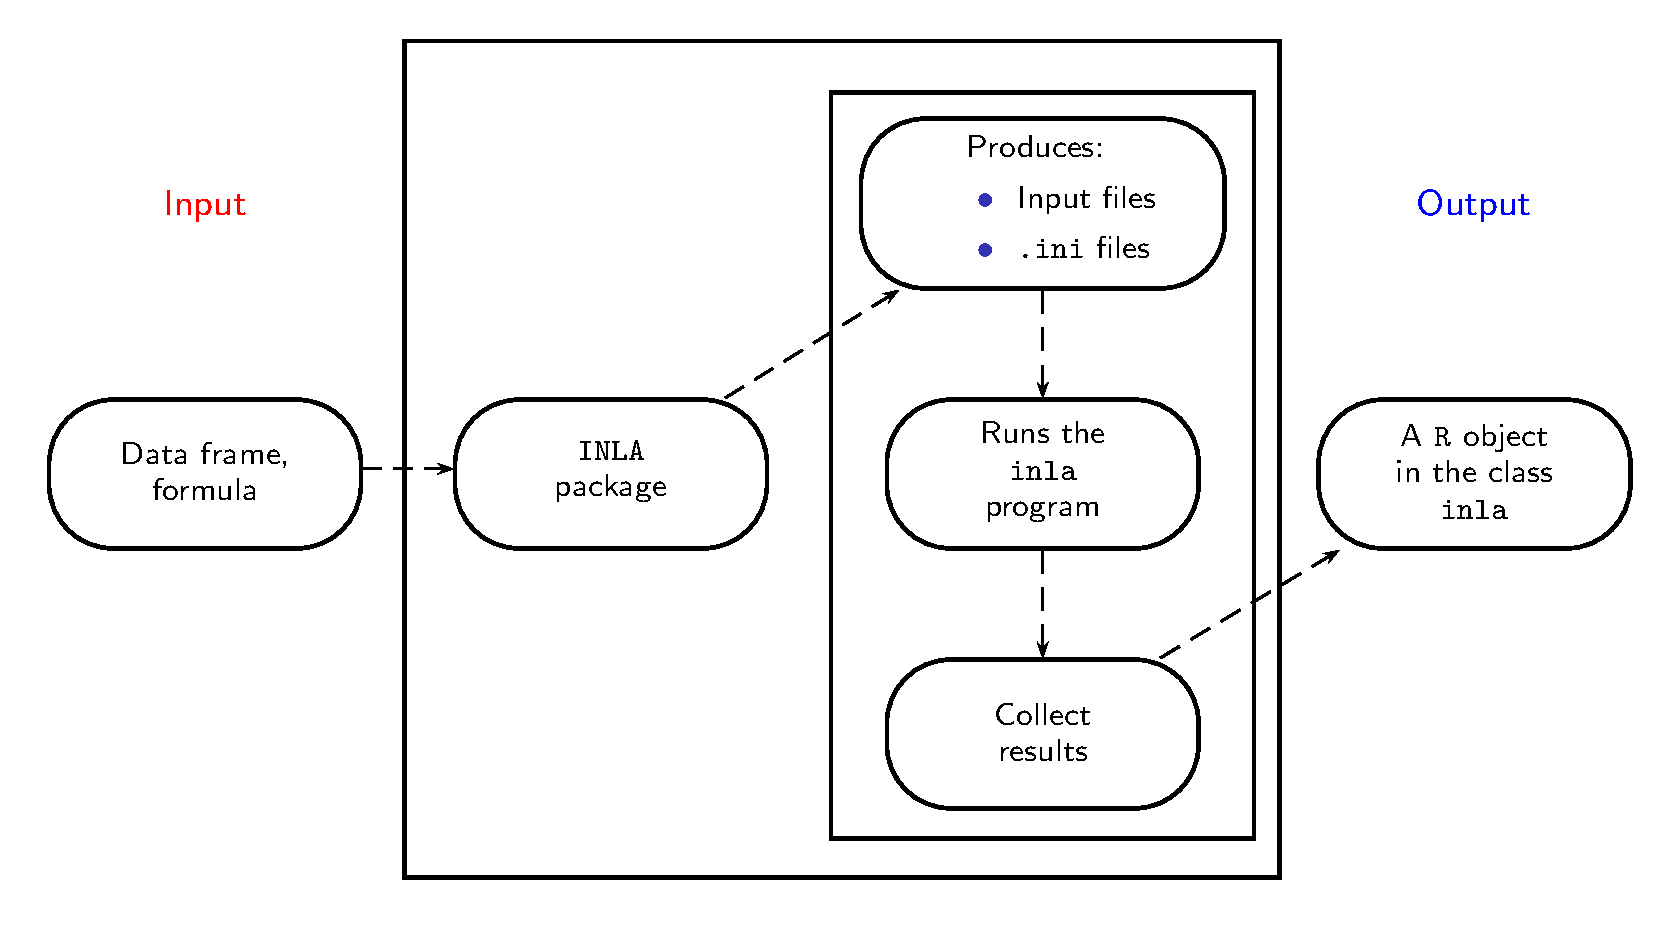
\includegraphics[width=1\linewidth]{graphics/inla-structure} \end{center}
\end{frame}

\begin{frame}[fragile]{What happens in the black box?}
\protect\hypertarget{what-happens-in-the-black-box}{}
The implementation of the INLA method consists of three parts:\\
\strut \\

\begin{itemize}
\item
  \textbf{GMRFLib-Library:} A library for GMRFs written in \texttt{C}
\item
  \textbf{\texttt{inla}-program:} The implementation of INLA written in
  \texttt{C}
\item
  \textbf{\texttt{INLA} package for \texttt{R}:} An \texttt{R}-interface
  to the \texttt{inla}-program\\
  \strut \\
  The first two are \emph{not} particularly user-friendly. They are used
  in the background by the \texttt{INLA} package.
\end{itemize}
\end{frame}

\begin{frame}[fragile]{Implementing INLA}
\protect\hypertarget{implementing-inla}{}
All procedures required to perform INLA need to be carefully implemented
to achieve a good speed; easier to implement a slow version of INLA.

\pause

\begin{itemize}
\item
  \textbf{The \texttt{GMRFLib}-library}

  \begin{itemize}
  \tightlist
  \item
    Basic library written in \texttt{C}, user friendly for programmers
  \end{itemize}
\end{itemize}
\end{frame}

\begin{frame}[fragile]{Implementing INLA}
\protect\hypertarget{implementing-inla-1}{}
All procedures required to perform INLA need to be carefully implemented
to achieve a good speed; easier to implement a slow version of INLA.

\begin{itemize}
\item
  \textbf{The \texttt{GMRFLib}-library}
\item
  \textbf{The \texttt{inla}-program}

  \begin{itemize}
  \tightlist
  \item
    Define \emph{latent Gaussian models} and interface with the
    \texttt{GMRFLib}-library
  \item
    Avoids the need for \texttt{C}-programming
  \item
    Models are defined using \texttt{.ini}-files
  \item
    Requires to write input files in a special format
  \item
    \texttt{inla}-program write all the results (E/Var/marginals) to
    files
  \end{itemize}
\end{itemize}
\end{frame}

\begin{frame}[fragile]{Implementing INLA}
\protect\hypertarget{implementing-inla-2}{}
All procedures required to perform INLA need to be carefully implemented
to achieve a good speed; easier to implement a slow version of INLA.

\begin{itemize}
\item
  \textbf{The \texttt{GMRFLib}-library}
\item
  \textbf{The \texttt{inla}-program}
\item
  \textbf{The \texttt{INLA} package for \texttt{R}}

  \begin{itemize}
  \tightlist
  \item
    \texttt{R}-interface to the \texttt{inla}-program. (That's why its
    not on CRAN.)
  \item
    Convert \texttt{formula}-statements into \texttt{.ini}-files
    definitions
  \item
    It also does much more (for example for survival models or when
    using \texttt{inlabru})
  \end{itemize}
\end{itemize}
\end{frame}

\hypertarget{how-to-use-inla}{%
\section{\texorpdfstring{How to use
\texttt{INLA}}{How to use INLA}}\label{how-to-use-inla}}

\begin{frame}[fragile]{How to use \texttt{INLA}}
\protect\hypertarget{how-to-use-inla-1}{}
There are essentially four parts to an \texttt{INLA}-program:\\
\strut \\
1. \textcolor{red}{Data organisation}: Make an object to store response,
covariates,

\begin{Shaded}
\begin{Highlighting}[]
\NormalTok{data }\OtherTok{=} \FunctionTok{data.fame}\NormalTok{(}\AttributeTok{y =}\NormalTok{ y, }\AttributeTok{x =}\NormalTok{ x)}
\end{Highlighting}
\end{Shaded}

\begin{enumerate}
\setcounter{enumi}{1}
\tightlist
\item
  \textcolor{red}{Use the `formula`-notation} to specify the model
  (similar to \texttt{lm} and \texttt{glm} functions)
\end{enumerate}

\begin{Shaded}
\begin{Highlighting}[]
\NormalTok{formula }\OtherTok{=}\NormalTok{ y}\SpecialCharTok{\textasciitilde{}}\NormalTok{x}
\end{Highlighting}
\end{Shaded}

\begin{enumerate}
\setcounter{enumi}{2}
\tightlist
\item
  \textcolor{red}{Call the `inla`-program}
\end{enumerate}

\begin{Shaded}
\begin{Highlighting}[]
\NormalTok{res }\OtherTok{=} \FunctionTok{inla}\NormalTok{(formula, }\AttributeTok{data=}\NormalTok{data, }\AttributeTok{family=}\StringTok{"gaussian"}\NormalTok{)}
\end{Highlighting}
\end{Shaded}

\begin{enumerate}
\setcounter{enumi}{3}
\tightlist
\item
  \textcolor{red}{Extract posterior information}, e.g.for a first
  overview use
\end{enumerate}

\begin{Shaded}
\begin{Highlighting}[]
\FunctionTok{summary}\NormalTok{(res)}
\end{Highlighting}
\end{Shaded}
\end{frame}

\begin{frame}[fragile]{Data organization}
\protect\hypertarget{data-organization}{}
The responses and covariates are collected in a
\textcolor{red}{list or data frame}. Assume response \texttt{y},
covariates \texttt{x1} and \texttt{x2}, and time index \texttt{t}. Then
they can be organized with:

\begin{Shaded}
\begin{Highlighting}[]
\CommentTok{\# Option 1}

\NormalTok{data }\OtherTok{=} \FunctionTok{list}\NormalTok{(}\AttributeTok{y =}\NormalTok{ y, }\AttributeTok{x1 =}\NormalTok{ x1, }\AttributeTok{x2 =}\NormalTok{ x2, }\AttributeTok{t =}\NormalTok{ t)}

\CommentTok{\# Option 2}

\NormalTok{data }\OtherTok{=} \FunctionTok{data.frame}\NormalTok{(}\AttributeTok{y =}\NormalTok{ y, }\AttributeTok{x1 =}\NormalTok{ x1, }\AttributeTok{x2 =}\NormalTok{ x2, }\AttributeTok{t =}\NormalTok{ t)}
\end{Highlighting}
\end{Shaded}
\end{frame}

\begin{frame}[fragile]{\texttt{formula}: specifying the linear
predictor}
\protect\hypertarget{formula-specifying-the-linear-predictor}{}
\textcolor{red}{The model is specified through a `formula`} similar to
\texttt{glm}:

\begin{Shaded}
\begin{Highlighting}[]
\NormalTok{formula }\OtherTok{=}\NormalTok{ y }\SpecialCharTok{\textasciitilde{}}\NormalTok{ x1 }\SpecialCharTok{+}\NormalTok{ x2 }\SpecialCharTok{+} \FunctionTok{f}\NormalTok{(t, ...)}
\end{Highlighting}
\end{Shaded}

\begin{itemize}
\item
  \texttt{y} is the name of the response in the \texttt{data} object
\item
  The fixed effects are given i.i.d. Gaussian priors
\item
  The \texttt{f()} function specifies random effects (e.g.~temporal,
  spatial, smooth effect of covariates and Besag model)
\item
  Use \texttt{-1} in the formula if you don't want an automatic
  intercept
\end{itemize}
\end{frame}

\begin{frame}[fragile]{The \texttt{inla()} function}
\protect\hypertarget{the-inla-function}{}
\small

\begin{Shaded}
\begin{Highlighting}[]
\NormalTok{result }\OtherTok{=} \FunctionTok{inla}\NormalTok{(}
  \CommentTok{\# Description of linear predictor}
\NormalTok{  formula,}
  \CommentTok{\# Likelihood}
  \AttributeTok{family =} \StringTok{"gaussian"}\NormalTok{,}
  \CommentTok{\# List or data frame with response, }
  \CommentTok{\# covariates, etc. }
  \AttributeTok{data =}\NormalTok{ data,}
  \DocumentationTok{\#\# This is all that is needed for a basic call }

  \DocumentationTok{\#\# \# check what happens}
  \AttributeTok{verbose =} \ConstantTok{TRUE}\NormalTok{,}
  \CommentTok{\# ,..., there are also some "control statements"}
  \CommentTok{\# to customize things}
  \CommentTok{\# This you need if you later want to sample from the}
  \CommentTok{\# fitted model}
  \AttributeTok{control.compute=}\FunctionTok{list}\NormalTok{(}\AttributeTok{config =} \ConstantTok{TRUE}\NormalTok{)}
\NormalTok{  )}
\end{Highlighting}
\end{Shaded}

\normalsize
\end{frame}

\begin{frame}[fragile]{Likelihood functions}
\protect\hypertarget{likelihood-functions}{}
\begin{itemize}
\item
  \texttt{gaussian}
\item
  \texttt{T}
\item
  \texttt{poisson}
\item
  \texttt{nbinomial}
\item
  \texttt{binomial}
\item
  \texttt{exponential}
\item
  \texttt{weibull}
\item
  \texttt{gev}
\item
  \texttt{coxph}
\end{itemize}

For a complete list type

\begin{Shaded}
\begin{Highlighting}[]
\FunctionTok{names}\NormalTok{(}\FunctionTok{inla.models}\NormalTok{()}\SpecialCharTok{$}\NormalTok{likelihood)}
\end{Highlighting}
\end{Shaded}
\end{frame}

\begin{frame}[fragile]{Posterior inference}
\protect\hypertarget{posterior-inference}{}
Main functions:

\begin{Shaded}
\begin{Highlighting}[]
\CommentTok{\# look at a  first summary}
\FunctionTok{summary}\NormalTok{(result)}
\CommentTok{\# plot the main results}
\CommentTok{\# (does not use ggplot...)}
\FunctionTok{plot}\NormalTok{(result)}
\CommentTok{\# rerun the model to get better}
\CommentTok{\# estimate of the hyperparemeters}
\NormalTok{result2 }\OtherTok{=} \FunctionTok{inla.hyperpar}\NormalTok{(result)}
\CommentTok{\# sample from the fitted model}
\CommentTok{\# this can be very useful sometimes!}
\NormalTok{sample }\OtherTok{=} \FunctionTok{inla.posterior.sample}\NormalTok{(results)}
\end{Highlighting}
\end{Shaded}
\end{frame}

\hypertarget{simple-example}{%
\section{Simple example}\label{simple-example}}

\begin{frame}{Example: Simple linear regression}
\protect\hypertarget{example-simple-linear-regression}{}
\begin{itemize}
\item
  \textbf{Stage 1:} Gaussian likelihood \[
  y_i | \eta_i \sim \mathcal{N}(\eta_i, \sigma^2)
  \]
\item
  \textbf{Stage 2:} Covariates are connected to likelihood by \[
  \eta_i = \beta_0 + \beta_1 x_i
  \]
\item
  \textbf{Stage 3:} \(\sigma^2\): variance of observation noise
\end{itemize}
\end{frame}

\begin{frame}[fragile]{Example: Simple linear regression}
\protect\hypertarget{example-simple-linear-regression-1}{}
\begin{Shaded}
\begin{Highlighting}[]
\CommentTok{\# Generate data}
\NormalTok{x }\OtherTok{=} \FunctionTok{runif}\NormalTok{(}\DecValTok{10}\NormalTok{)}
\NormalTok{y }\OtherTok{=} \DecValTok{1} \SpecialCharTok{+} \DecValTok{2}\SpecialCharTok{*}\NormalTok{x }\SpecialCharTok{+} \FunctionTok{rnorm}\NormalTok{(}\AttributeTok{n =} \DecValTok{100}\NormalTok{, }\AttributeTok{sd =} \FloatTok{0.1}\NormalTok{)}

\CommentTok{\# Run inla}
\NormalTok{formula }\OtherTok{=}\NormalTok{ y }\SpecialCharTok{\textasciitilde{}} \DecValTok{1} \SpecialCharTok{+}\NormalTok{ x}
\NormalTok{result }\OtherTok{=} \FunctionTok{inla}\NormalTok{(formula,}
              \AttributeTok{data =} \FunctionTok{data.frame}\NormalTok{(}\AttributeTok{x =}\NormalTok{ x, }\AttributeTok{y =}\NormalTok{ y),}
              \AttributeTok{family =} \StringTok{"gaussian"}\NormalTok{)}
\end{Highlighting}
\end{Shaded}
\end{frame}

\begin{frame}[fragile]{Organization of the \texttt{inla}-object}
\protect\hypertarget{organization-of-the-inla-object}{}
\tiny

\begin{Shaded}
\begin{Highlighting}[]
\FunctionTok{names}\NormalTok{(result)}
\end{Highlighting}
\end{Shaded}

\begin{verbatim}
##  [1] "names.fixed"                 "summary.fixed"              
##  [3] "marginals.fixed"             "summary.lincomb"            
##  [5] "marginals.lincomb"           "size.lincomb"               
##  [7] "summary.lincomb.derived"     "marginals.lincomb.derived"  
##  [9] "size.lincomb.derived"        "mlik"                       
## [11] "cpo"                         "po"                         
## [13] "waic"                        "model.random"               
## [15] "summary.random"              "marginals.random"           
## [17] "size.random"                 "summary.linear.predictor"   
## [19] "marginals.linear.predictor"  "summary.fitted.values"      
## [21] "marginals.fitted.values"     "size.linear.predictor"      
## [23] "summary.hyperpar"            "marginals.hyperpar"         
## [25] "internal.summary.hyperpar"   "internal.marginals.hyperpar"
## [27] "offset.linear.predictor"     "model.spde2.blc"            
## [29] "summary.spde2.blc"           "marginals.spde2.blc"        
## [31] "size.spde2.blc"              "model.spde3.blc"            
## [33] "summary.spde3.blc"           "marginals.spde3.blc"        
## [35] "size.spde3.blc"              "logfile"                    
## [37] "misc"                        "dic"                        
## [39] "mode"                        "joint.hyper"                
## [41] "nhyper"                      "version"                    
## [43] "Q"                           "graph"                      
## [45] "ok"                          "cpu.used"                   
## [47] "all.hyper"                   ".args"                      
## [49] "call"                        "model.matrix"
\end{verbatim}

\normalsize
\end{frame}

\begin{frame}[fragile]{Organization of the \texttt{inla}-object}
\protect\hypertarget{organization-of-the-inla-object-1}{}
You can find summary information in \small

\begin{verbatim}
##  [1] "summary.fixed"             "summary.lincomb"          
##  [3] "summary.lincomb.derived"   "summary.random"           
##  [5] "summary.linear.predictor"  "summary.fitted.values"    
##  [7] "summary.hyperpar"          "internal.summary.hyperpar"
##  [9] "summary.spde2.blc"         "summary.spde3.blc"
\end{verbatim}

\normalsize

for example

\scriptsize

\begin{Shaded}
\begin{Highlighting}[]
\NormalTok{result}\SpecialCharTok{$}\NormalTok{summary.fixed}
\end{Highlighting}
\end{Shaded}

\begin{verbatim}
##                 mean         sd 0.025quant 0.5quant 0.975quant     mode
## (Intercept) 1.002781 0.01981293  0.9638022 1.002780   1.041726 1.002781
## x           1.974175 0.03346575  1.9083371 1.974174   2.039957 1.974175
##                      kld
## (Intercept) 3.086520e-06
## x           3.086389e-06
\end{verbatim}

\normalsize
\end{frame}

\begin{frame}[fragile]{Organization of the \texttt{inla}-object}
\protect\hypertarget{organization-of-the-inla-object-2}{}
You can find estimated posterior marginals in \small

\begin{verbatim}
##  [1] "marginals.fixed"             "marginals.lincomb"          
##  [3] "marginals.lincomb.derived"   "marginals.random"           
##  [5] "marginals.linear.predictor"  "marginals.fitted.values"    
##  [7] "marginals.hyperpar"          "internal.marginals.hyperpar"
##  [9] "marginals.spde2.blc"         "marginals.spde3.blc"
\end{verbatim}

\normalsize

Each object is thereby a list. Get the marginal for intercept:

\scriptsize

\begin{Shaded}
\begin{Highlighting}[]
   \FunctionTok{head}\NormalTok{(result}\SpecialCharTok{$}\NormalTok{marginals.fixed[[}\DecValTok{1}\NormalTok{]])}
\end{Highlighting}
\end{Shaded}

\begin{verbatim}
##              x            y
## [1,] 0.8043030 2.146677e-17
## [2,] 0.8439985 3.450320e-11
## [3,] 0.8836940 1.944195e-06
## [4,] 0.8941229 2.290543e-05
## [5,] 0.9035418 1.840298e-04
## [6,] 0.9043623 2.192137e-04
\end{verbatim}

\normalsize
\end{frame}

\begin{frame}[fragile]{Organization of the \texttt{inla}-object}
\protect\hypertarget{organization-of-the-inla-object-3}{}
Further general information

\begin{Shaded}
\begin{Highlighting}[]
\CommentTok{\# formula used}
\NormalTok{result}\SpecialCharTok{$}\NormalTok{.args}\SpecialCharTok{$}\NormalTok{formula}
\end{Highlighting}
\end{Shaded}

\begin{verbatim}
## y ~ 1 + x
## NULL
\end{verbatim}

\begin{Shaded}
\begin{Highlighting}[]
\CommentTok{\# data used}
\NormalTok{result}\SpecialCharTok{$}\NormalTok{.args}\SpecialCharTok{$}\NormalTok{data[}\DecValTok{1}\SpecialCharTok{:}\DecValTok{3}\NormalTok{,]}
\end{Highlighting}
\end{Shaded}

\begin{verbatim}
##           x        y
## 1 0.8051767 2.617140
## 2 0.7827668 2.542227
## 3 0.1807834 1.157771
\end{verbatim}

\begin{Shaded}
\begin{Highlighting}[]
\CommentTok{\# log{-}file including information of INLA approximations}
\NormalTok{result}\SpecialCharTok{$}\NormalTok{logfile}
\end{Highlighting}
\end{Shaded}
\end{frame}

\begin{frame}[fragile]{Marginal posterior densities}
\protect\hypertarget{marginal-posterior-densities}{}
The marginal posterior densities are stored as a matrices with \(x\)-
and \(y\)-values \small

\begin{Shaded}
\begin{Highlighting}[]
\NormalTok{intercept }\OtherTok{=} \FunctionTok{data.frame}\NormalTok{(result}\SpecialCharTok{$}\NormalTok{marginals.fixed}\SpecialCharTok{$}\StringTok{\textasciigrave{}}\AttributeTok{(Intercept)}\StringTok{\textasciigrave{}}\NormalTok{)}
\NormalTok{x }\OtherTok{=} \FunctionTok{data.frame}\NormalTok{(result}\SpecialCharTok{$}\NormalTok{marginals.fixed}\SpecialCharTok{$}\NormalTok{x)}
\NormalTok{p1 }\OtherTok{=} \FunctionTok{ggplot}\NormalTok{(}\AttributeTok{data =}\NormalTok{ intercept) }\SpecialCharTok{+} \FunctionTok{geom\_point}\NormalTok{(}\FunctionTok{aes}\NormalTok{(x,y))}
\NormalTok{p2 }\OtherTok{=} \FunctionTok{ggplot}\NormalTok{(}\AttributeTok{data =}\NormalTok{ x) }\SpecialCharTok{+} \FunctionTok{geom\_point}\NormalTok{(}\FunctionTok{aes}\NormalTok{(x,y))}
\NormalTok{p1}\SpecialCharTok{+}\NormalTok{p2}
\end{Highlighting}
\end{Shaded}

\begin{center}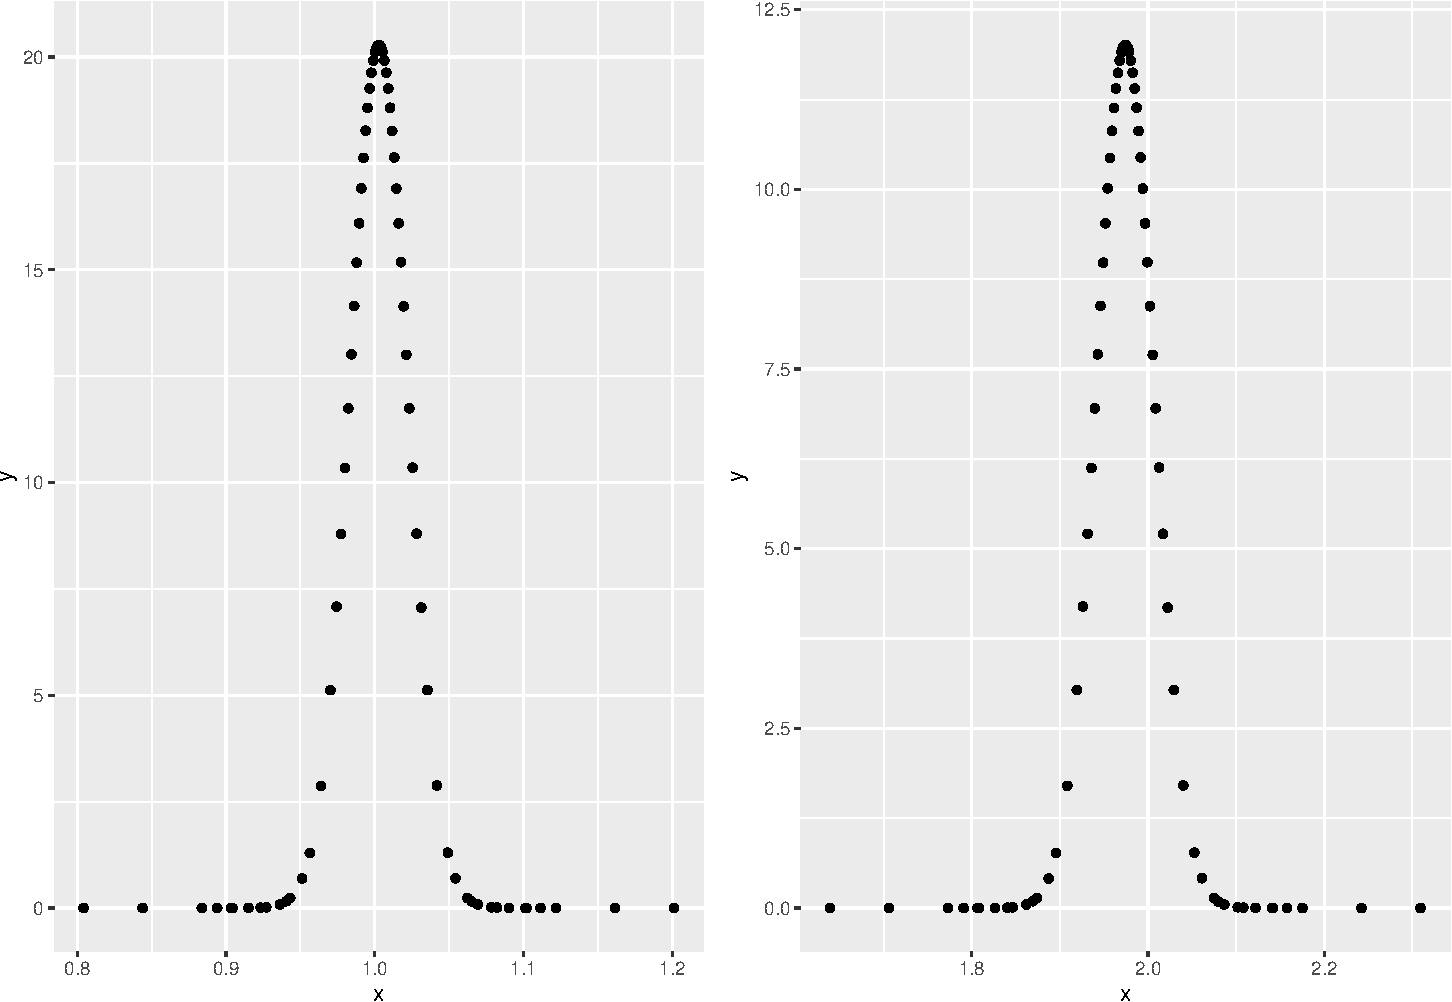
\includegraphics[width=0.6\linewidth]{Part2_RINLA_files/figure-beamer/unnamed-chunk-25-1} \end{center}
\normalsize
\end{frame}

\begin{frame}[fragile]{Marginal posterior densities}
\protect\hypertarget{marginal-posterior-densities-1}{}
The rough shape can be interpolated to higher resolution using the
\texttt{inla.smarginal()} function:

\begin{Shaded}
\begin{Highlighting}[]
\NormalTok{smoother\_dens }\OtherTok{=} \FunctionTok{data.frame}\NormalTok{(}\FunctionTok{inla.smarginal}\NormalTok{(intercept))}
\FunctionTok{ggplot}\NormalTok{(}\AttributeTok{data =}\NormalTok{ smoother\_dens) }\SpecialCharTok{+} \FunctionTok{geom\_point}\NormalTok{(}\FunctionTok{aes}\NormalTok{(x,y))}
\end{Highlighting}
\end{Shaded}

\begin{center}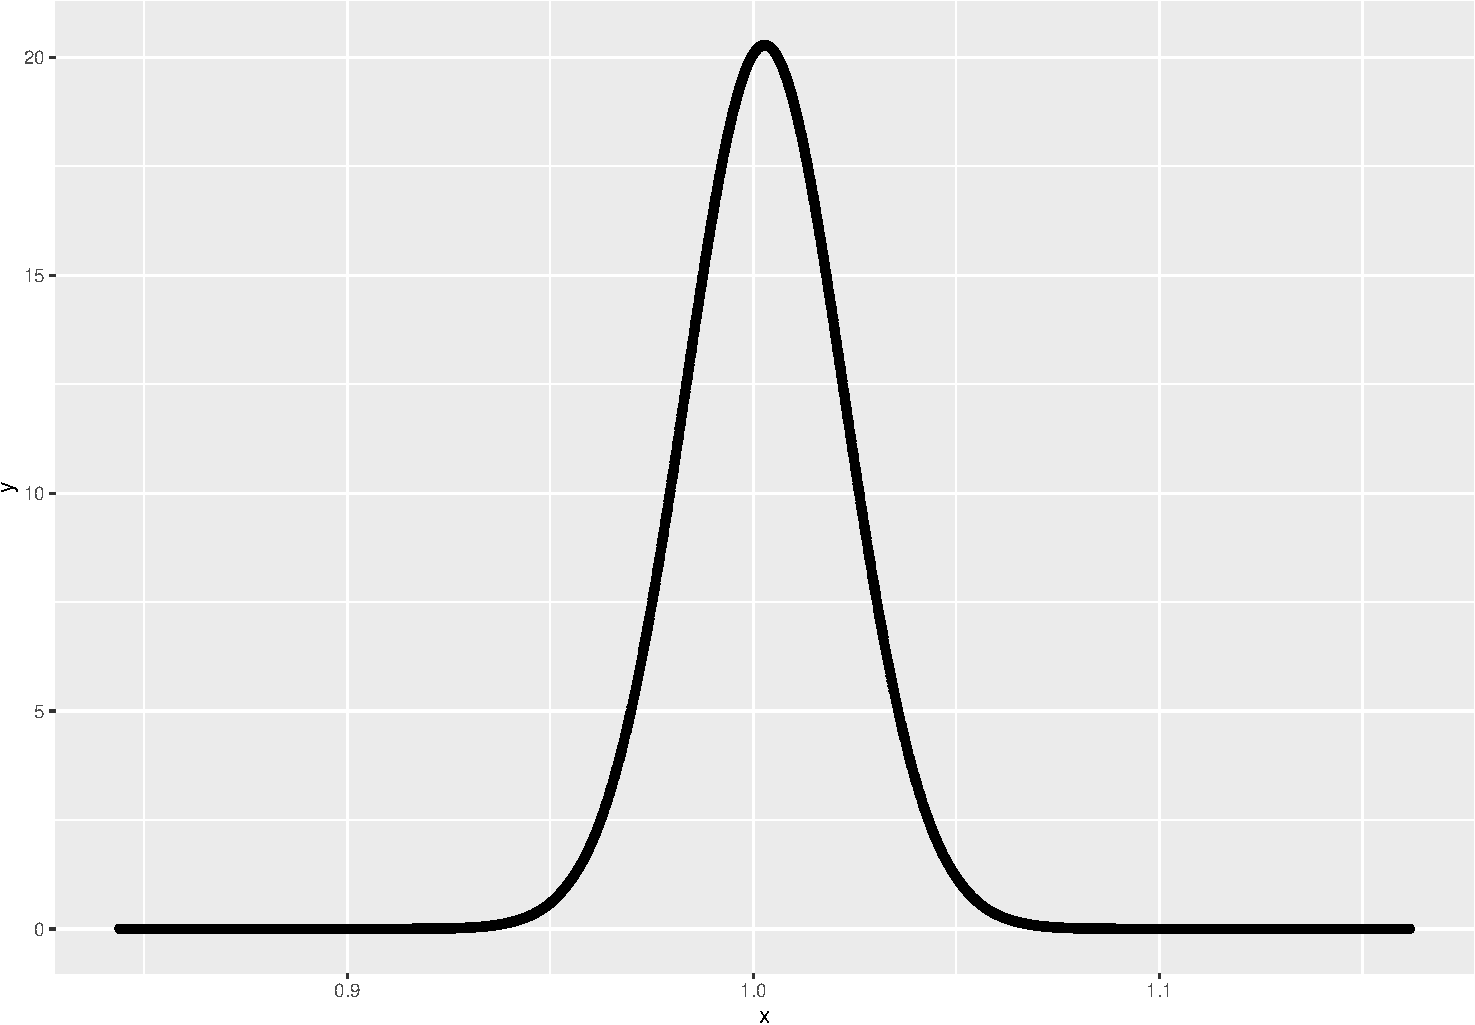
\includegraphics[width=0.6\linewidth]{Part2_RINLA_files/figure-beamer/unnamed-chunk-26-1} \end{center}
\end{frame}

\begin{frame}[fragile]{Marginal posterior densities}
\protect\hypertarget{marginal-posterior-densities-2}{}
Manipulation of the computed posterior marginals is possible through the
\texttt{inla.*marginal()} functions:

\small

\begin{Shaded}
\begin{Highlighting}[]
\CommentTok{\# compute the 0.05 quantile}
\FunctionTok{inla.qmarginal}\NormalTok{(}\FloatTok{0.05}\NormalTok{, intercept)}
\end{Highlighting}
\end{Shaded}

\begin{verbatim}
## [1] 0.9701406
\end{verbatim}

\begin{Shaded}
\begin{Highlighting}[]
\CommentTok{\# Distribution function}
\FunctionTok{inla.pmarginal}\NormalTok{(}\FloatTok{0.975}\NormalTok{, intercept)}
\end{Highlighting}
\end{Shaded}

\begin{verbatim}
## [1] 0.08047574
\end{verbatim}

\begin{Shaded}
\begin{Highlighting}[]
\CommentTok{\# Density function}
\FunctionTok{inla.dmarginal}\NormalTok{(}\DecValTok{1}\NormalTok{, intercept)}
\end{Highlighting}
\end{Shaded}

\begin{verbatim}
## [1] 20.07664
\end{verbatim}

\begin{Shaded}
\begin{Highlighting}[]
\CommentTok{\# Generate realizations}
\FunctionTok{inla.rmarginal}\NormalTok{(}\DecValTok{4}\NormalTok{, intercept)}
\end{Highlighting}
\end{Shaded}

\begin{verbatim}
## [1] 0.9969020 1.0146015 1.0341315 0.9967547
\end{verbatim}

\normalsize
\end{frame}

\begin{frame}{Other \texttt{inla.*marginal()} functions.}
\protect\hypertarget{other-inla.marginal-functions.}{}
\scriptsize
\begin{table}[h]
\centering
    \begin{tabular}{l|p{6cm}}
     \bf{Function Name} & \bf{Usage}\\\hline\hline
      \tt{inla.dmarginal(x, marginal, $\dots$)} & Density at a vector of
      evaluation  \\
      & points $x$ \\
      \tt{inla.pmarginal(q, marginal, $\dots$)} & Distribution function at a vector  \\
      &  of
      quantiles $q$ \\
      \tt{inla.qmarginal(p, marginal, $\dots$)} & Quantile function at a vector \\
      & of
      probabilities $p$.\\
      \tt{inla.rmarginal(n, marginal)} & Generate $n$ random deviates \\
      \tt{inla.hpdmarginal(p, marginal, $\dots$)} & Compute the highest posterior \\
      & density
      interval at level $p$\\
      \tt{inla.emarginal(fun, marginal, $\dots$)} & Compute the expected value \\
      & of the
      marginal assuming the transformation given by fun\\
      \tt{inla.mmarginal(marginal)} & Compute the mode\\
      \tt{inla.smarginal(marginal, $\dots$)} & Smoothed density in
      form of a list of length two. The first entry contains the x-values, the second
      entry includes the interpolated y-values\\
      \tt{inla.tmarginal(fun, marginal, $\dots$)} & Transform the marginal using the
      function fun.\\
      \tt{inla.zmarginal(marginal)} & Summary statistics for the marginal\\
    \end{tabular}
\end{table}
\normalsize
\end{frame}

\hypertarget{add-random-effects}{%
\section{Add random effects}\label{add-random-effects}}

\begin{frame}[fragile]{Add random effects}
\protect\hypertarget{add-random-effects-1}{}
\begin{Shaded}
\begin{Highlighting}[]
\FunctionTok{f}\NormalTok{(name, }\AttributeTok{model=}\StringTok{"..."}\NormalTok{, }\AttributeTok{hyper=}\NormalTok{...,}
                 \AttributeTok{constr=}\ConstantTok{FALSE}\NormalTok{, }\AttributeTok{cyclic=}\ConstantTok{FALSE}\NormalTok{, ...)}
\end{Highlighting}
\end{Shaded}

\begin{itemize}
\tightlist
\item
  \texttt{name} -- the index of the effect
  (\textcolor{red}{each f-function needs its own!})
\item
  \texttt{model} -- the type of latent model. E.g.\texttt{iid},
  \texttt{rw2}, \texttt{ar1}, \texttt{besag}, and so on
\item
  \texttt{hyper} -- specify the prior on the hyperparameters
\item
  \texttt{constr} -- sum-to-zero constraint?
\item
  \texttt{cyclic} -- are you cyclic?
\item
  \texttt{...}
\end{itemize}
\end{frame}

\begin{frame}{Example: Add random effect}
\protect\hypertarget{example-add-random-effect}{}
Add an AR(1) random effect to the linear predictor.

\begin{itemize}
\item
  \textbf{Stage 1:} \[
    y_i|\eta_i \sim \mathcal{N}(\eta_i, \sigma^2)
  \]
\item
  \textbf{Stage 2:} Covariates and AR(1) component connected to
  likelihood by
\end{itemize}

\[
    \eta_i = \beta_0 + \beta_1 x_i + a_i
\]

\begin{itemize}
\item
  \textbf{Stage 3:}

  \begin{itemize}
  \item
    \(\sigma^2\): variance of observation noise
  \item
    \(\rho\): dependence in AR(1) process
  \item
    \(\sigma^2\): variance of the innovations in AR(1) process
  \end{itemize}
\end{itemize}
\end{frame}

\begin{frame}[fragile]{Example: Add random effect}
\protect\hypertarget{example-add-random-effect-1}{}
\small

\begin{Shaded}
\begin{Highlighting}[]
\CommentTok{\# Generate AR(1) sequence}
\FunctionTok{set.seed}\NormalTok{(}\DecValTok{580258}\NormalTok{)}
\NormalTok{t }\OtherTok{=} \DecValTok{1}\SpecialCharTok{:}\DecValTok{100}
\NormalTok{rho }\OtherTok{=} \FloatTok{0.8}
\NormalTok{sd\_ar1 }\OtherTok{=} \FloatTok{0.1}
\NormalTok{ar }\OtherTok{=} \FunctionTok{rep}\NormalTok{(}\DecValTok{0}\NormalTok{,}\DecValTok{100}\NormalTok{)}
\ControlFlowTok{for}\NormalTok{(i }\ControlFlowTok{in} \DecValTok{2}\SpecialCharTok{:}\DecValTok{100}\NormalTok{)}
\NormalTok{  ar[i] }\OtherTok{=}\NormalTok{ rho }\SpecialCharTok{*}\NormalTok{ ar[i}\DecValTok{{-}1}\NormalTok{] }\SpecialCharTok{+} \FunctionTok{rnorm}\NormalTok{(}\AttributeTok{n =} \DecValTok{1}\NormalTok{, }\AttributeTok{sd =}\NormalTok{ sd\_ar1)}
\CommentTok{\# Generate data with AR(1) component}
\NormalTok{x }\OtherTok{=} \FunctionTok{runif}\NormalTok{(}\DecValTok{100}\NormalTok{)}
\NormalTok{y }\OtherTok{=} \DecValTok{1} \SpecialCharTok{+} \DecValTok{2}\SpecialCharTok{*}\NormalTok{x }\SpecialCharTok{+}\NormalTok{ ar }\SpecialCharTok{+} \FunctionTok{rnorm}\NormalTok{(}\AttributeTok{n =} \DecValTok{100}\NormalTok{, }\AttributeTok{sd =} \FloatTok{0.2}\NormalTok{)}

\CommentTok{\# Run inla}
\NormalTok{formula }\OtherTok{=}\NormalTok{ y }\SpecialCharTok{\textasciitilde{}} \DecValTok{1} \SpecialCharTok{+}\NormalTok{ x }\SpecialCharTok{+} \FunctionTok{f}\NormalTok{(t, }\AttributeTok{model=}\StringTok{"ar1"}\NormalTok{)}

\NormalTok{result }\OtherTok{=} \FunctionTok{inla}\NormalTok{(formula,}
     \AttributeTok{data =} \FunctionTok{data.frame}\NormalTok{(}\AttributeTok{x =}\NormalTok{ x, }\AttributeTok{y =}\NormalTok{ y, }\AttributeTok{t =}\NormalTok{ t),}
     \AttributeTok{family =} \StringTok{"gaussian"}\NormalTok{)}
\end{Highlighting}
\end{Shaded}

\normalsize
\end{frame}

\begin{frame}[fragile]{Example}
\protect\hypertarget{example}{}
Estimates of the random effect \small

\begin{Shaded}
\begin{Highlighting}[]
\NormalTok{result}\SpecialCharTok{$}\NormalTok{summary.random}\SpecialCharTok{$}\NormalTok{t }\SpecialCharTok{\%\textgreater{}\%} \FunctionTok{ggplot}\NormalTok{() }\SpecialCharTok{+}
  \FunctionTok{geom\_line}\NormalTok{(}\FunctionTok{aes}\NormalTok{(ID, mean)) }\SpecialCharTok{+} 
  \FunctionTok{geom\_ribbon}\NormalTok{(}\FunctionTok{aes}\NormalTok{(ID, }\AttributeTok{ymin =} \StringTok{\textasciigrave{}}\AttributeTok{0.025quant}\StringTok{\textasciigrave{}}\NormalTok{, }\AttributeTok{ymax =} \StringTok{\textasciigrave{}}\AttributeTok{0.975quant}\StringTok{\textasciigrave{}}\NormalTok{), }\AttributeTok{alpha =} \FloatTok{0.3}\NormalTok{) }\SpecialCharTok{+}
  \FunctionTok{geom\_point}\NormalTok{(}\AttributeTok{data =} \FunctionTok{data.frame}\NormalTok{(}\AttributeTok{t =}\NormalTok{t , }\AttributeTok{ar =}\NormalTok{ ar), }\FunctionTok{aes}\NormalTok{(t,ar), }\AttributeTok{color =} \StringTok{"red"}\NormalTok{)}
\end{Highlighting}
\end{Shaded}

\begin{center}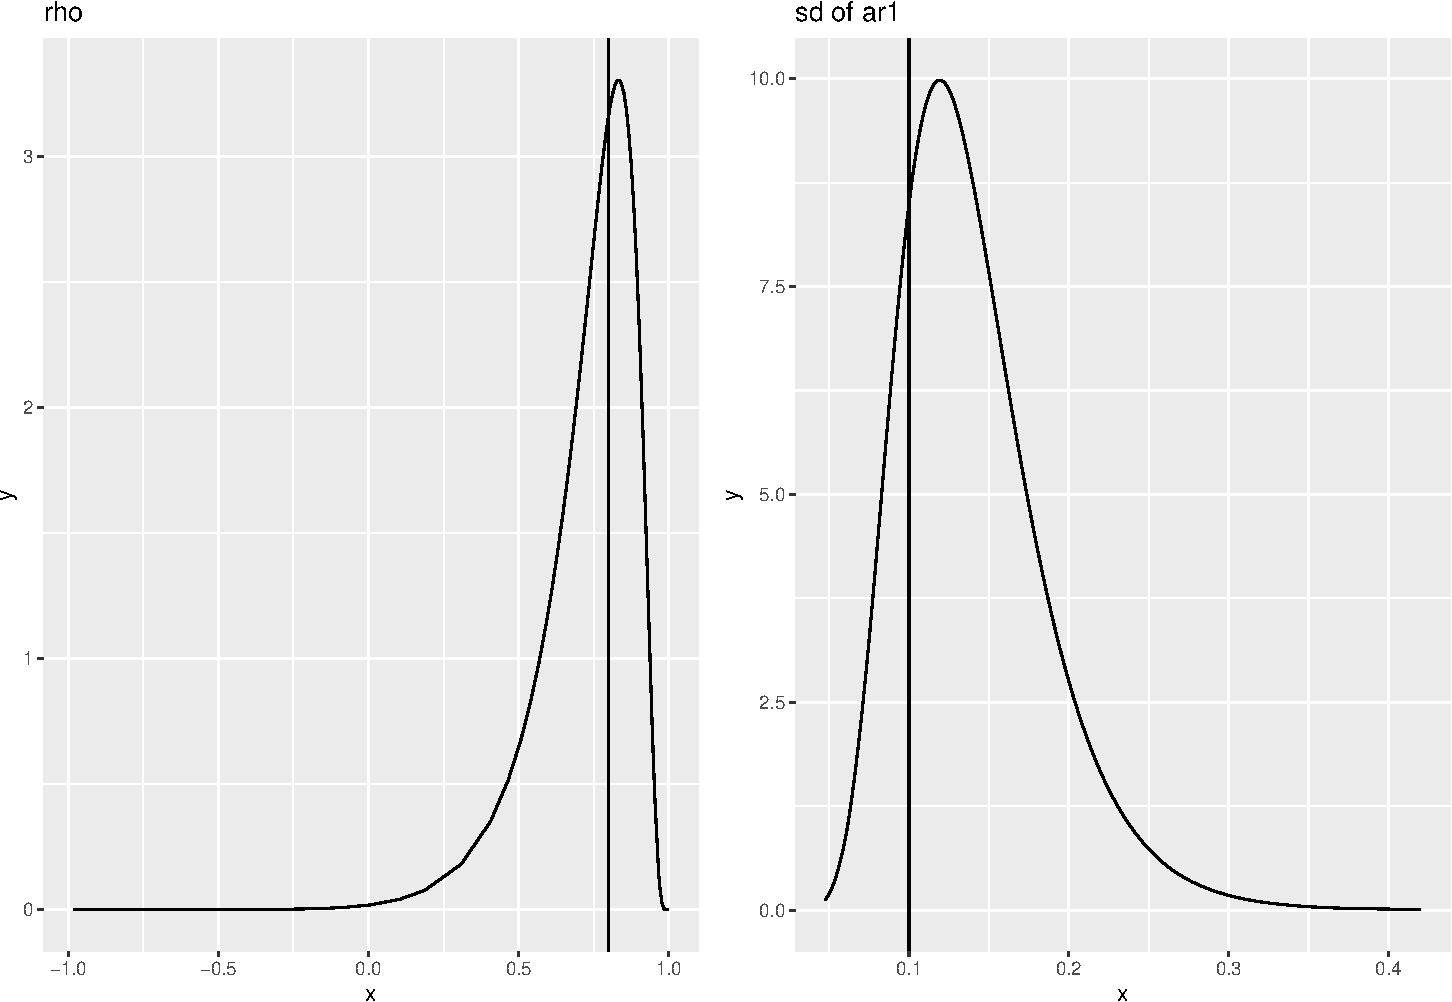
\includegraphics[width=0.6\linewidth]{Part2_RINLA_files/figure-beamer/unnamed-chunk-33-1} \end{center}
\normalsize
\end{frame}

\begin{frame}[fragile]{Example}
\protect\hypertarget{example-1}{}
Estimates of the hyperparameters \footnotesize

\begin{Shaded}
\begin{Highlighting}[]
\CommentTok{\# rho }
\NormalTok{p1 }\OtherTok{=} \FunctionTok{ggplot}\NormalTok{() }\SpecialCharTok{+} \FunctionTok{geom\_line}\NormalTok{(}\AttributeTok{data =} \FunctionTok{data.frame}\NormalTok{(result}\SpecialCharTok{$}\NormalTok{marginals.hyperpar}\SpecialCharTok{$}\StringTok{\textasciigrave{}}\AttributeTok{Rho for t}\StringTok{\textasciigrave{}}\NormalTok{), }
                          \FunctionTok{aes}\NormalTok{(x,y)) }\SpecialCharTok{+}
  \FunctionTok{geom\_vline}\NormalTok{(}\AttributeTok{xintercept =}\NormalTok{ rho) }\SpecialCharTok{+} \FunctionTok{ggtitle}\NormalTok{(}\StringTok{"rho"}\NormalTok{)}
\CommentTok{\# sd of the ar1 effect}
\NormalTok{prec }\OtherTok{=}\NormalTok{ result}\SpecialCharTok{$}\NormalTok{marginals.hyperpar}\SpecialCharTok{$}\StringTok{\textasciigrave{}}\AttributeTok{Precision for t}\StringTok{\textasciigrave{}}
\NormalTok{sd }\OtherTok{=} \FunctionTok{inla.tmarginal}\NormalTok{(}\ControlFlowTok{function}\NormalTok{(x) }\DecValTok{1}\SpecialCharTok{/}\FunctionTok{sqrt}\NormalTok{(x), prec)}
\NormalTok{p2 }\OtherTok{=} \FunctionTok{ggplot}\NormalTok{() }\SpecialCharTok{+} \FunctionTok{geom\_line}\NormalTok{(}\AttributeTok{data =} \FunctionTok{data.frame}\NormalTok{(sd), }\FunctionTok{aes}\NormalTok{(x,y)) }\SpecialCharTok{+}
  \FunctionTok{geom\_vline}\NormalTok{(}\AttributeTok{xintercept =}\NormalTok{sd\_ar1 ) }\SpecialCharTok{+} \FunctionTok{ggtitle}\NormalTok{(}\StringTok{"sd of ar1"}\NormalTok{)}
\NormalTok{p1}\SpecialCharTok{+}\NormalTok{p2}
\end{Highlighting}
\end{Shaded}

\begin{center}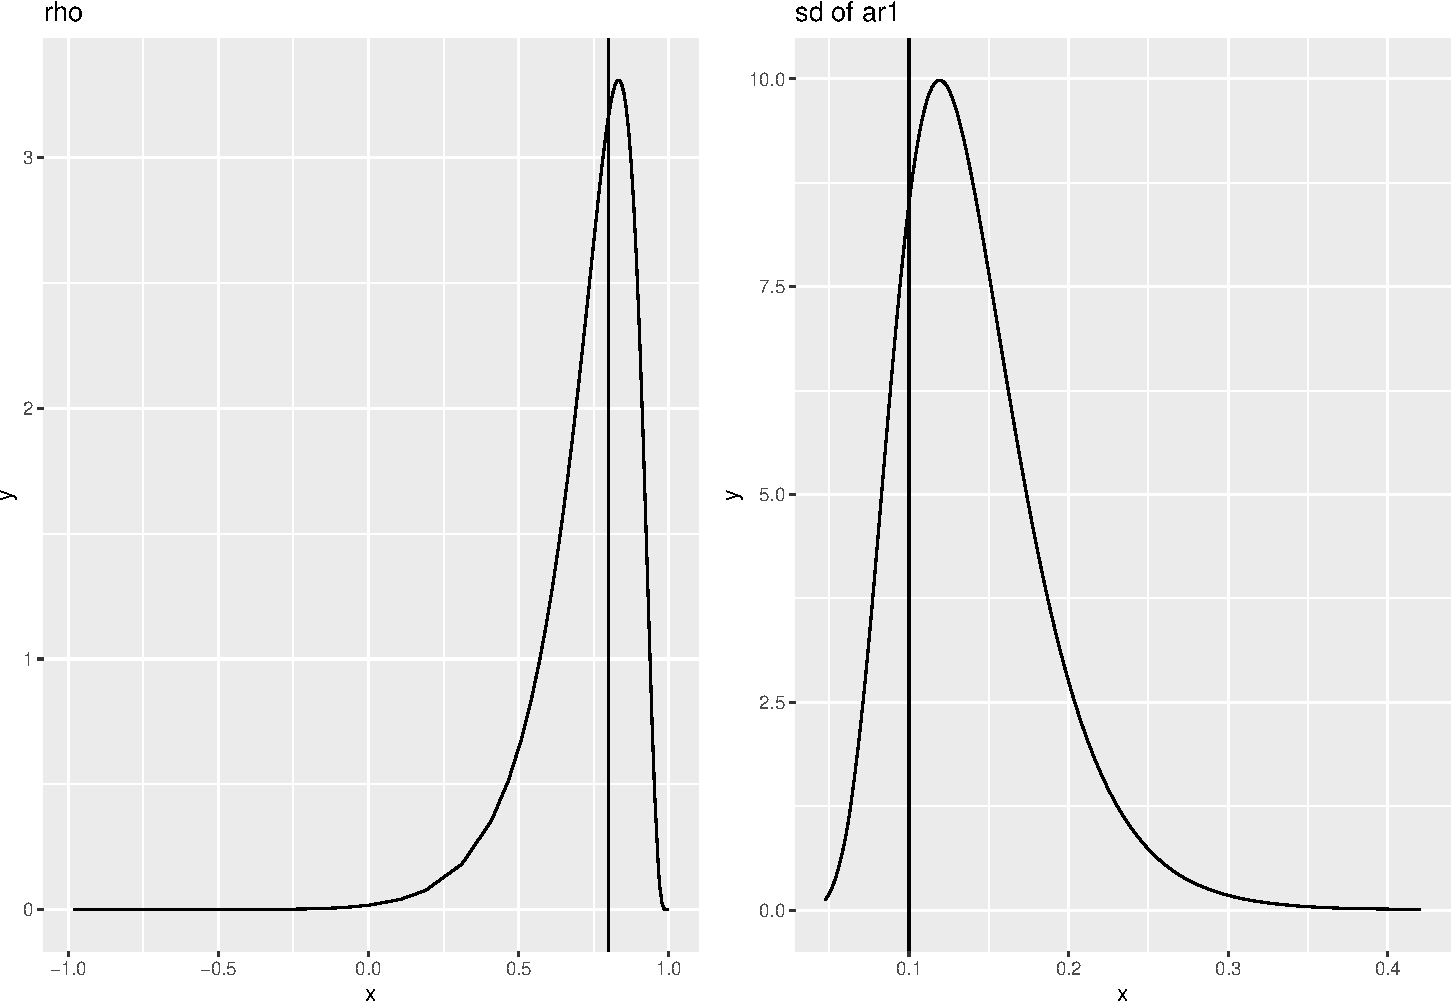
\includegraphics[width=0.4\linewidth]{Part2_RINLA_files/figure-beamer/unnamed-chunk-34-1} \end{center}
\end{frame}

\hypertarget{prediction}{%
\section{Prediction}\label{prediction}}

\begin{frame}[fragile]{The interpretation of \texttt{NA}}
\protect\hypertarget{the-interpretation-of-na}{}
\texttt{R-INLA} uses \texttt{NA} differently than other packages

\begin{itemize}
\item
  \texttt{NA} in the \textbf{response} means no likelihood contribution,
  i.e.response is unobserved
\item
  \texttt{NA} in a \textbf{fixed effect} means no contribution to the
  linear predictor, i.e.~the covariate is set equal to zero
\item
  \texttt{NA} in a \textbf{random effect} \texttt{f(...)} means no
  contribution to the linear predictor
\end{itemize}
\end{frame}

\begin{frame}[fragile]{Prediction}
\protect\hypertarget{prediction-1}{}
The distribution of the linear predictor at an unobserved location can
be computed by specifying the value of the covariate \(x\) and the
desired time index \(t\) and set \(y\) to \texttt{NA}. \small

\begin{Shaded}
\begin{Highlighting}[]
\CommentTok{\# Add one new location}
\NormalTok{n }\OtherTok{=} \DecValTok{1}
\NormalTok{x }\OtherTok{=} \FunctionTok{c}\NormalTok{(x, }\FunctionTok{runif}\NormalTok{(n))}
\NormalTok{t }\OtherTok{=} \FunctionTok{c}\NormalTok{(t, }\DecValTok{101}\SpecialCharTok{:}\NormalTok{(}\DecValTok{100}\SpecialCharTok{+}\NormalTok{n))}
\NormalTok{y }\OtherTok{=} \FunctionTok{c}\NormalTok{(y, }\FunctionTok{rep}\NormalTok{(}\ConstantTok{NA}\NormalTok{,n))}

\CommentTok{\# Re{-}compute}
\NormalTok{result.pred }\OtherTok{=} \FunctionTok{inla}\NormalTok{(formula,}
    \AttributeTok{data =} \FunctionTok{data.frame}\NormalTok{(}\AttributeTok{x =}\NormalTok{ x, }\AttributeTok{t =}\NormalTok{ t, }\AttributeTok{y =}\NormalTok{ y),}
    \AttributeTok{family=}\StringTok{"gaussian"}\NormalTok{,}
    \AttributeTok{control.inla =} \FunctionTok{list}\NormalTok{(}\AttributeTok{int.strategy =} \StringTok{"grid"}\NormalTok{),}
    \AttributeTok{control.compute =} \FunctionTok{list}\NormalTok{(}\AttributeTok{config =} \ConstantTok{TRUE}\NormalTok{, }
                           \AttributeTok{return.marginals.predictor=}\ConstantTok{TRUE}\NormalTok{), }
    \CommentTok{\# tell inla to return the marginals for eta!  }
    \AttributeTok{control.predictor =} \FunctionTok{list}\NormalTok{(}\AttributeTok{compute =} \ConstantTok{TRUE}\NormalTok{))}
\end{Highlighting}
\end{Shaded}

\normalsize
\end{frame}

\begin{frame}[fragile]{Prediction}
\protect\hypertarget{prediction-2}{}
Predicted marginal of the linear predictor \(\eta_{101}\)

\begin{Shaded}
\begin{Highlighting}[]
\NormalTok{pred }\OtherTok{=}\NormalTok{ result.pred}\SpecialCharTok{$}\NormalTok{marginals.linear.predictor[[}\DecValTok{100}\SpecialCharTok{+}\NormalTok{n]]}
\NormalTok{pred }\OtherTok{=} \FunctionTok{inla.smarginal}\NormalTok{(pred)}
\FunctionTok{ggplot}\NormalTok{() }\SpecialCharTok{+}
  \FunctionTok{geom\_line}\NormalTok{(}\AttributeTok{data =} \FunctionTok{data.frame}\NormalTok{(pred), }\FunctionTok{aes}\NormalTok{(x, y)) }
\end{Highlighting}
\end{Shaded}

\begin{center}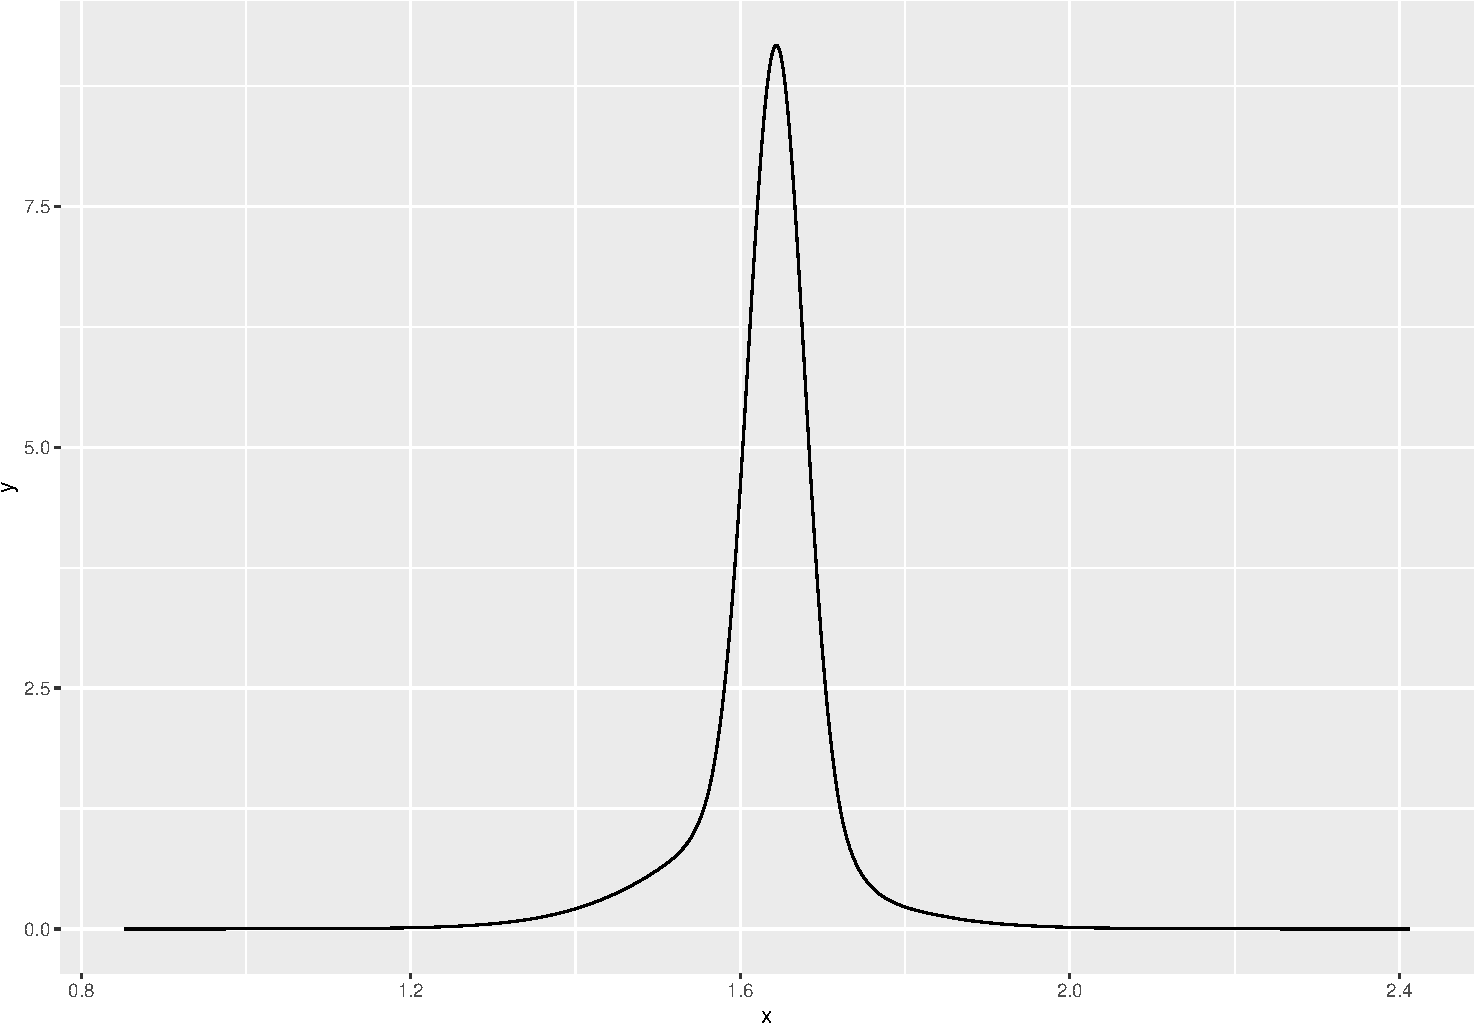
\includegraphics[width=0.6\linewidth]{Part2_RINLA_files/figure-beamer/unnamed-chunk-36-1} \end{center}
\end{frame}

\begin{frame}{Prediction}
\protect\hypertarget{prediction-3}{}
\textcolor{red}{Caution}: This is \textbf{not} yet the predictive
distribution, as the observation noise is missing.

The predictive distribution is \[
\pi(y_{101}|\bf{y})
\] what we got is \[
\pi(\eta_{101}|\bf{y})
\]
\end{frame}

\begin{frame}[fragile]{Prediction}
\protect\hypertarget{prediction-4}{}
One way to add the observation noise to the linear predictor is by
sampling from the posterior distribution.

\small

\begin{Shaded}
\begin{Highlighting}[]
\NormalTok{n }\OtherTok{=} \DecValTok{1000}
\NormalTok{x }\OtherTok{=} \FunctionTok{inla.posterior.sample}\NormalTok{(n, result.pred)}

\NormalTok{func }\OtherTok{=} \ControlFlowTok{function}\NormalTok{(...)}
\NormalTok{\{}
\NormalTok{  eta }\OtherTok{=}\NormalTok{ Predictor}
\NormalTok{  eta }\OtherTok{=}\NormalTok{ eta[}\DecValTok{101}\NormalTok{]}
\NormalTok{  sd }\OtherTok{=} \DecValTok{1}\SpecialCharTok{/}\FunctionTok{sqrt}\NormalTok{(theta[}\DecValTok{1}\NormalTok{])}
\NormalTok{  out }\OtherTok{=} \FunctionTok{rnorm}\NormalTok{(}\DecValTok{1}\NormalTok{, }\AttributeTok{mean =}\NormalTok{ eta, }\AttributeTok{sd =}\NormalTok{sd)}
  \FunctionTok{return}\NormalTok{(out)}
\NormalTok{\}}

\NormalTok{samples }\OtherTok{=} \FunctionTok{inla.posterior.sample.eval}\NormalTok{(func, x)[}\DecValTok{1}\NormalTok{,]}
\end{Highlighting}
\end{Shaded}
\end{frame}

\begin{frame}{Prediction}
\protect\hypertarget{prediction-5}{}
Comparing \(\pi(y_{101}|\bf{y})\) and \(\pi(\eta_{101}|\bf{y})\)

\begin{center}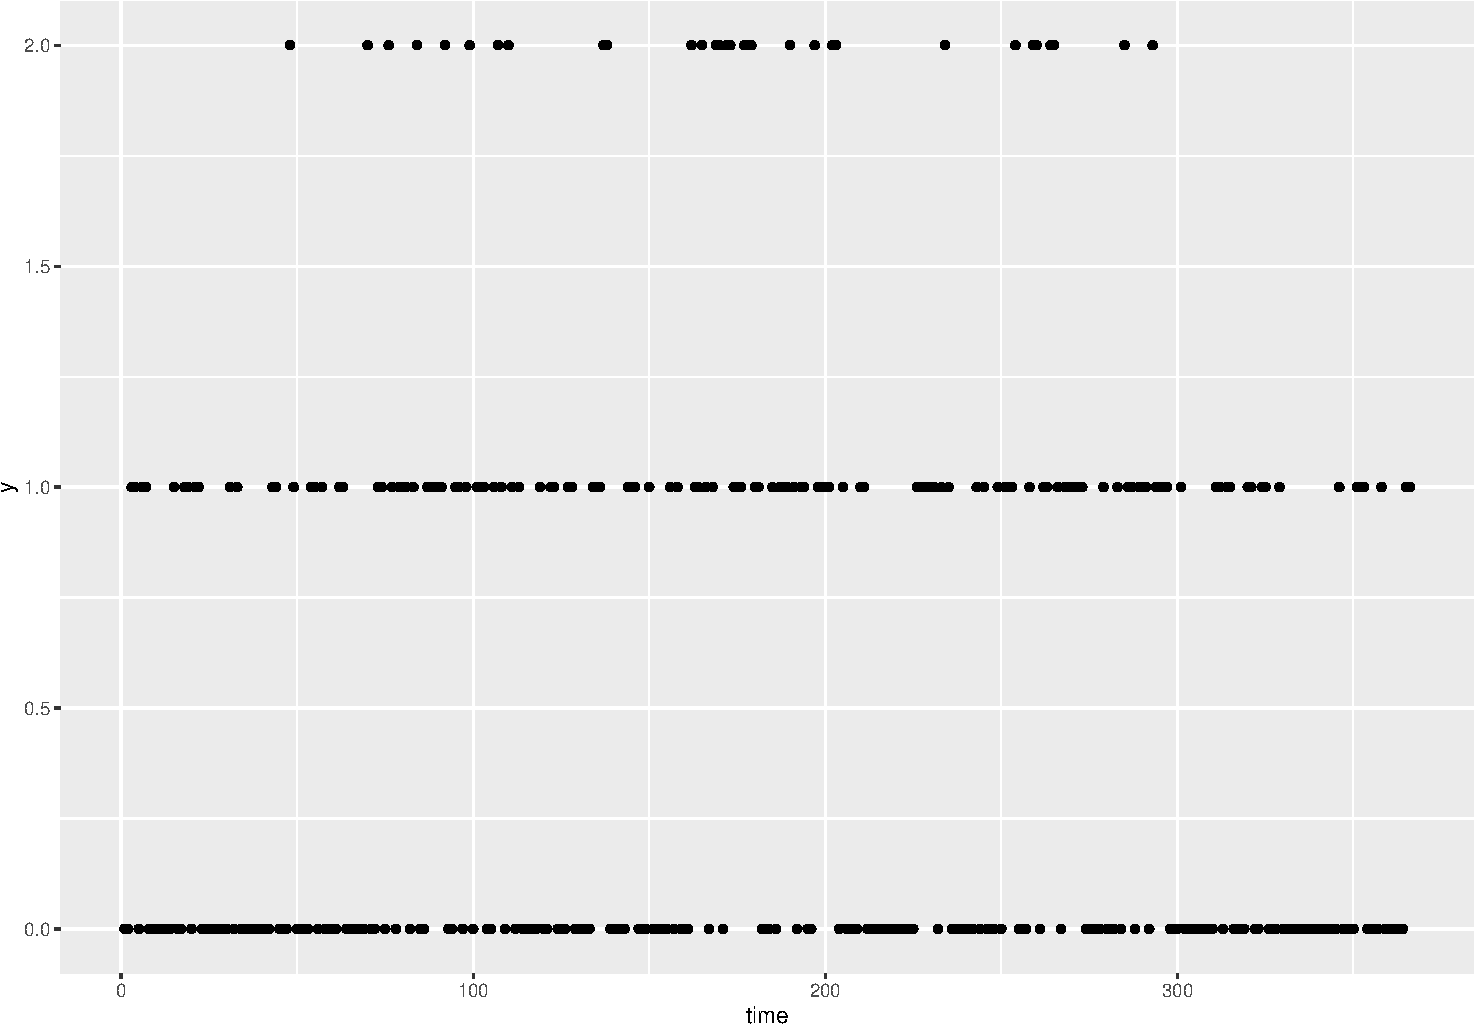
\includegraphics[width=0.6\linewidth]{Part2_RINLA_files/figure-beamer/unnamed-chunk-37-1} \end{center}
\normalsize
\end{frame}

\hypertarget{smoothing-binary-time-series}{%
\section{Smoothing binary time
series}\label{smoothing-binary-time-series}}

\begin{frame}[fragile]{Example: Smoothing binary time series}
\protect\hypertarget{example-smoothing-binary-time-series}{}
The data set \texttt{Tokyo} is available in the \texttt{INLA} package
and consists of the number of days in Tokyo with rainfall above 1 mm in
1983--1984.

\begin{center}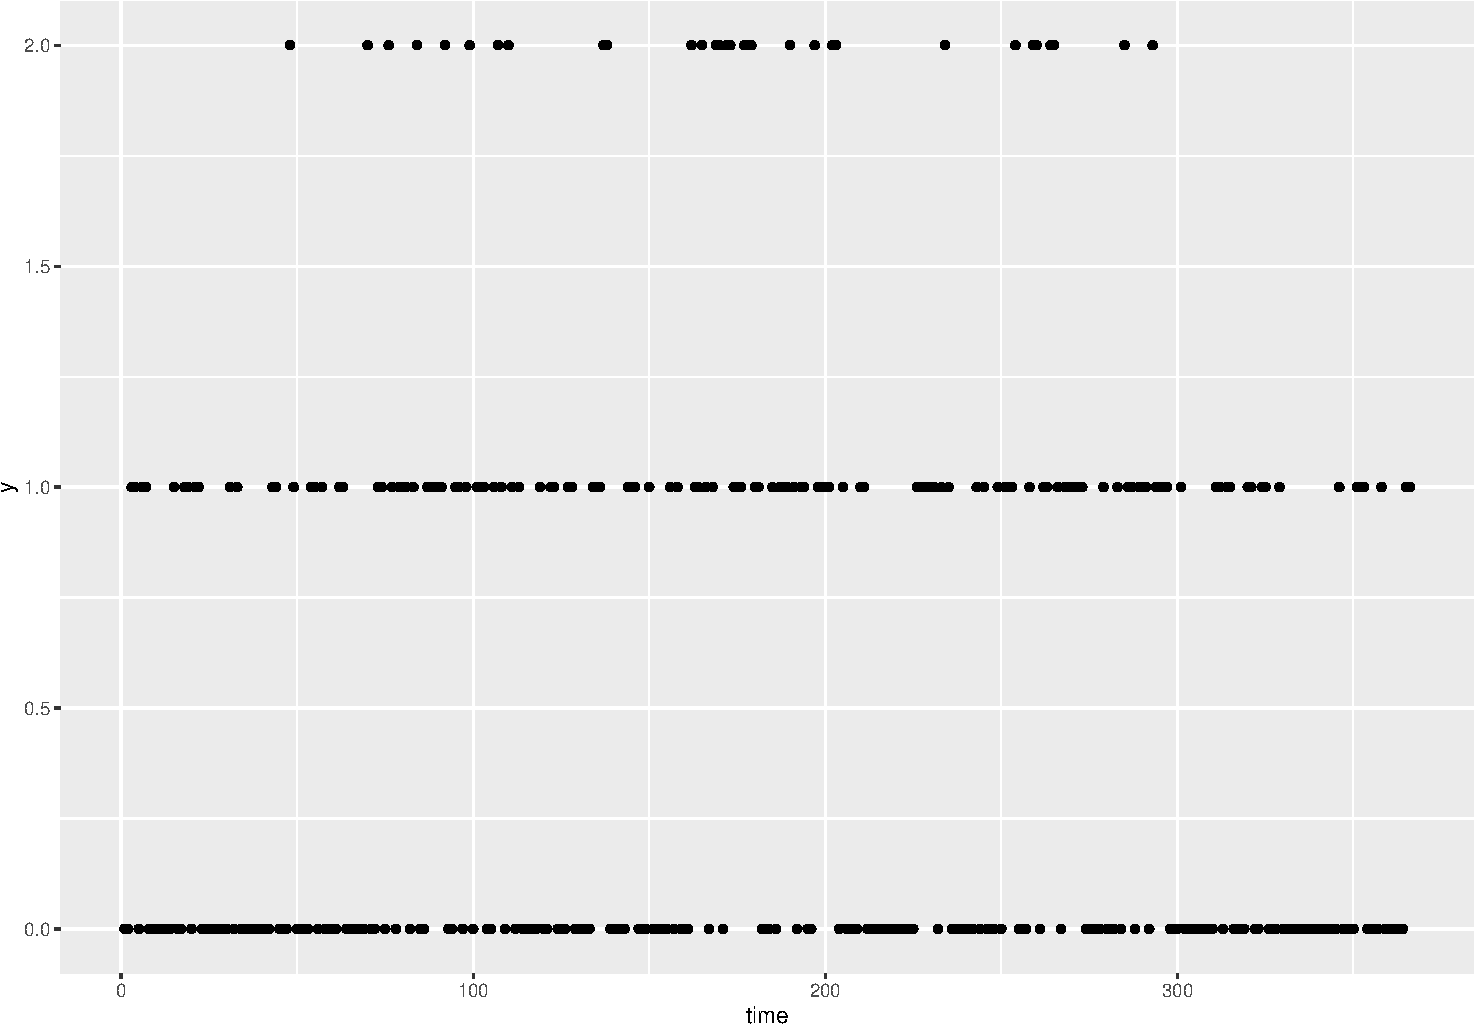
\includegraphics[width=0.6\linewidth]{Part2_RINLA_files/figure-beamer/unnamed-chunk-38-1} \end{center}
\end{frame}

\begin{frame}[fragile]{Observations}
\protect\hypertarget{observations}{}
Each observation consists of

\begin{itemize}
\item
  \(t\): Day of year; \(t\in\{1,2,\ldots, 366\}\)
\item
  \(n_t\): Number of observations for day \(t\) in 1983--1984;
  \(n_t\in\{1,2\}\)
\item
  \(y_t\): Number of days with rain out of \(n_t\) days for day \(t\);
  \(y_t \in \{0, 1, 2\}\)
\end{itemize}

\footnotesize

\begin{Shaded}
\begin{Highlighting}[]
 \FunctionTok{data}\NormalTok{(Tokyo)}
\FunctionTok{head}\NormalTok{(Tokyo,}\DecValTok{3}\NormalTok{)}
\end{Highlighting}
\end{Shaded}

\begin{verbatim}
##   y n time
## 1 0 2    1
## 2 0 2    2
## 3 1 2    3
\end{verbatim}

\begin{Shaded}
\begin{Highlighting}[]
\NormalTok{Tokyo[}\DecValTok{60}\NormalTok{,]}
\end{Highlighting}
\end{Shaded}

\begin{verbatim}
##    y n time
## 60 0 1   60
\end{verbatim}

\normalsize
\end{frame}

\begin{frame}{Hierarchical model}
\protect\hypertarget{hierarchical-model}{}
\begin{itemize}
\item
  \textbf{Stage 1:} We have binomial responses with known \(n_t\), but
  unknown probabilities \[
  y_t \sim \text{Binomial}(n_t, p_t)
  \]
\item
  \textbf{Stage 2:} A cyclic second order random walk (CRW2) is
  connected to the likelihood by \[
  p_t = \frac{\exp{(\eta_t})}{1+\exp(\eta_t)}\, \text{with linear predictor}\,\eta_t = \mathrm{CRW2}_t
  \]
\item
  \textbf{Stage 3:}

  \begin{itemize}
  \tightlist
  \item
    \(\tau\): Scale parameter in CRW2 with prior \[
        \pi(\tau) \sim \text{Gamma}(1, 5\cdot 10^{-5})
    \]
  \end{itemize}
\end{itemize}
\end{frame}

\begin{frame}[fragile]{\texttt{INLA} implementation}
\protect\hypertarget{inla-implementation}{}
\begin{Shaded}
\begin{Highlighting}[]
\CommentTok{\# Read data}
\FunctionTok{data}\NormalTok{(Tokyo)}
\CommentTok{\# Specify linear predictor}
\NormalTok{formula }\OtherTok{=}\NormalTok{ y }\SpecialCharTok{\textasciitilde{}} \SpecialCharTok{{-}}\DecValTok{1} \SpecialCharTok{+} \FunctionTok{f}\NormalTok{(time, }\AttributeTok{model=}\StringTok{"rw2"}\NormalTok{, }\AttributeTok{cyclic=}\ConstantTok{TRUE}\NormalTok{)}
\CommentTok{\# Run model}
\NormalTok{result }\OtherTok{=} \FunctionTok{inla}\NormalTok{(formula,}
              \AttributeTok{family =} \StringTok{"binomial"}\NormalTok{,}
              \AttributeTok{Ntrials =}\NormalTok{ n,}
              \AttributeTok{data =}\NormalTok{ Tokyo)}
\end{Highlighting}
\end{Shaded}
\end{frame}

\begin{frame}[fragile]{Marginal posterior of CRW2}
\protect\hypertarget{marginal-posterior-of-crw2}{}
\begin{Shaded}
\begin{Highlighting}[]
\FunctionTok{ggplot}\NormalTok{(}\AttributeTok{data =}\NormalTok{ result}\SpecialCharTok{$}\NormalTok{summary.random}\SpecialCharTok{$}\NormalTok{t) }\SpecialCharTok{+} 
  \FunctionTok{geom\_line}\NormalTok{(}\FunctionTok{aes}\NormalTok{(ID, mean)) }\SpecialCharTok{+}
  \FunctionTok{geom\_ribbon}\NormalTok{(}\FunctionTok{aes}\NormalTok{(ID, }\AttributeTok{ymin =} \StringTok{\textasciigrave{}}\AttributeTok{0.025quant}\StringTok{\textasciigrave{}}\NormalTok{, }\AttributeTok{ymax =} \StringTok{\textasciigrave{}}\AttributeTok{0.975quant}\StringTok{\textasciigrave{}}\NormalTok{ ),}
              \AttributeTok{alpha =} \FloatTok{0.5}\NormalTok{)}
\end{Highlighting}
\end{Shaded}

\begin{center}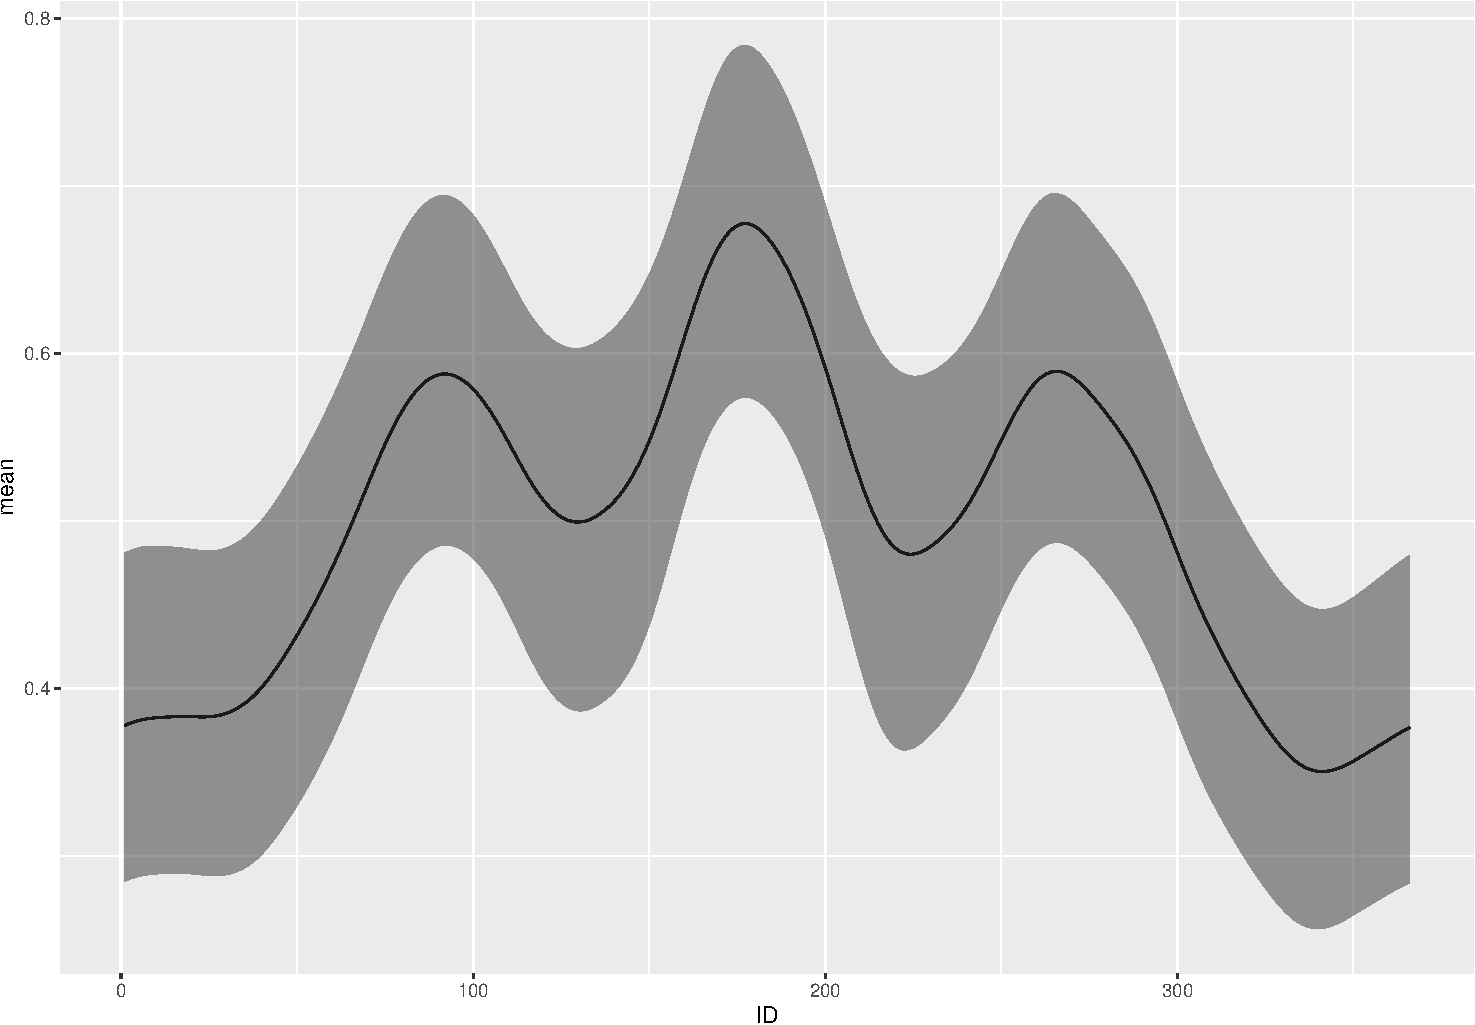
\includegraphics[width=0.6\linewidth]{Part2_RINLA_files/figure-beamer/unnamed-chunk-42-1} \end{center}
\end{frame}

\begin{frame}[fragile]{Transform to probability}
\protect\hypertarget{transform-to-probability}{}
\small

\begin{Shaded}
\begin{Highlighting}[]
\NormalTok{pred }\OtherTok{=}\NormalTok{ result}\SpecialCharTok{$}\NormalTok{summary.fitted.values}
\NormalTok{pred}\SpecialCharTok{$}\NormalTok{ID }\OtherTok{=} \DecValTok{1}\SpecialCharTok{:}\FunctionTok{dim}\NormalTok{(Tokyo)[}\DecValTok{1}\NormalTok{]}
\FunctionTok{ggplot}\NormalTok{(}\AttributeTok{data =}\NormalTok{ pred) }\SpecialCharTok{+} 
  \FunctionTok{geom\_line}\NormalTok{(}\FunctionTok{aes}\NormalTok{(ID, mean)) }\SpecialCharTok{+}
  \FunctionTok{geom\_ribbon}\NormalTok{(}\FunctionTok{aes}\NormalTok{(ID, }\AttributeTok{ymin =} \StringTok{\textasciigrave{}}\AttributeTok{0.025quant}\StringTok{\textasciigrave{}}\NormalTok{, }\AttributeTok{ymax =} \StringTok{\textasciigrave{}}\AttributeTok{0.975quant}\StringTok{\textasciigrave{}}\NormalTok{ ),}
              \AttributeTok{alpha =} \FloatTok{0.5}\NormalTok{)}
\end{Highlighting}
\end{Shaded}

\begin{center}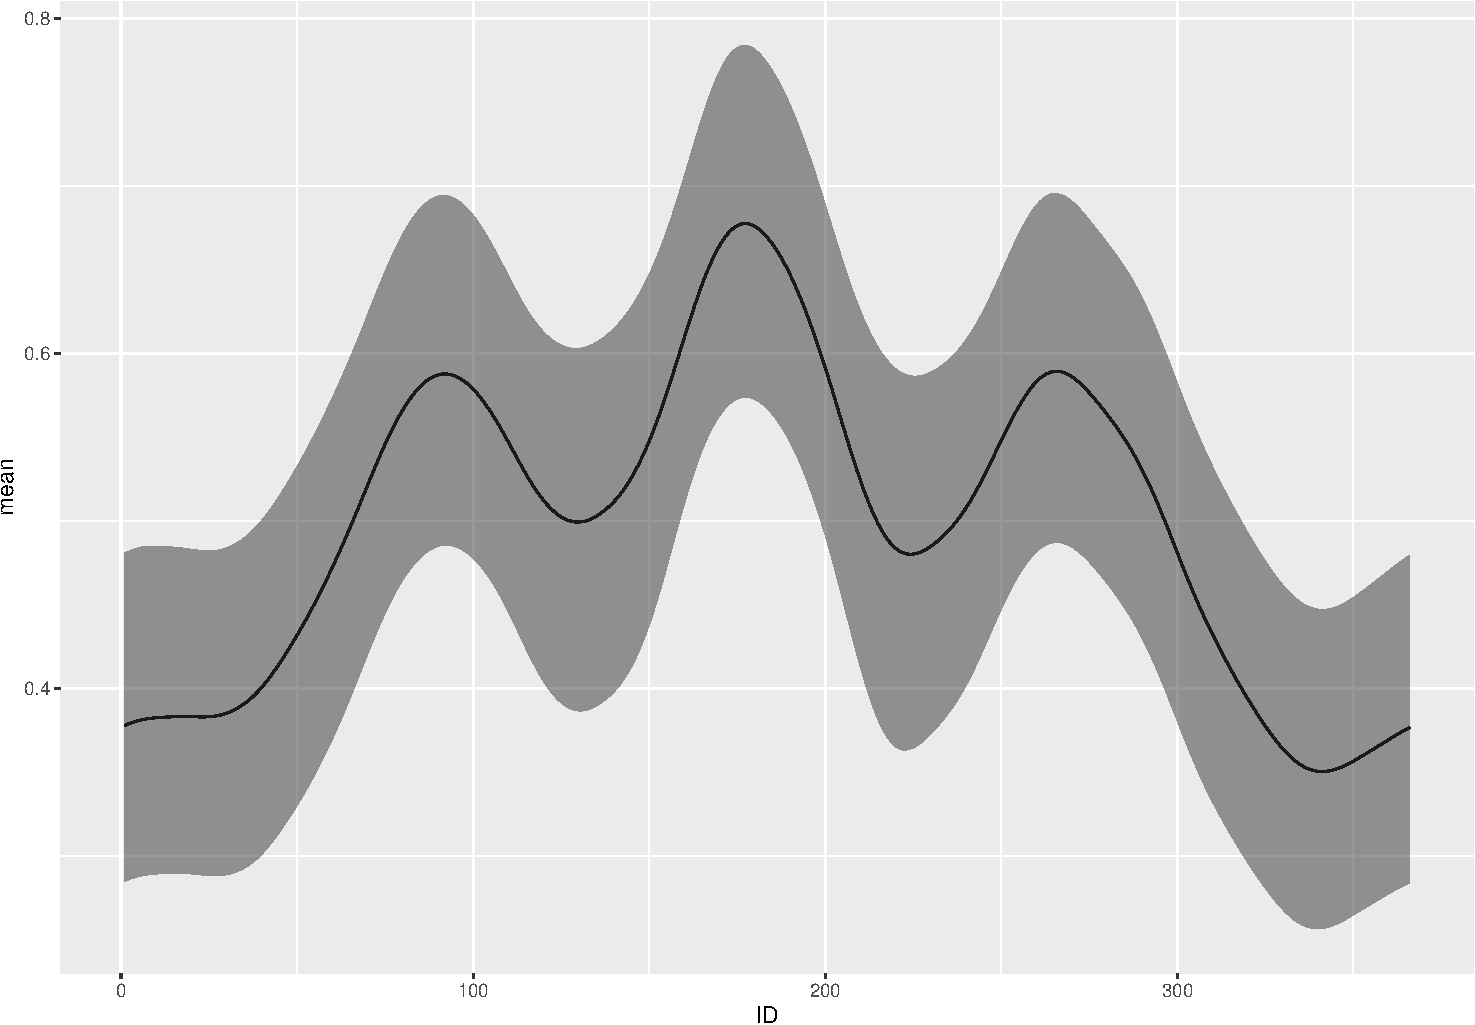
\includegraphics[width=0.6\linewidth]{Part2_RINLA_files/figure-beamer/unnamed-chunk-43-1} \end{center}
\normalsize
\end{frame}

\hypertarget{disease-mapping}{%
\section{Disease Mapping}\label{disease-mapping}}

\begin{frame}{Example: disease mapping}
\protect\hypertarget{example-disease-mapping}{}
We observed larynx cancer mortality counts for males in 544 district of
Germany from 1986 to 1990 and want to make a model.

\begin{cols}

\begin{col}{0.55\textwidth}

\begin{itemize}
\tightlist
\item
  \(y_i\): The count at location \(i\).
\item
  \(E_i\): An offset; expected number of cases in district \(i\).
\item
  \(c_i\): A covariate (level of smoking consumption) at \(i\)
\item
  \(\boldsymbol{s}_i\): spatial location \(i\) .
\end{itemize}

\end{col}

\begin{col}{0.05\textwidth}
~

\end{col}

\begin{col}{0.4\textwidth}

\begin{center}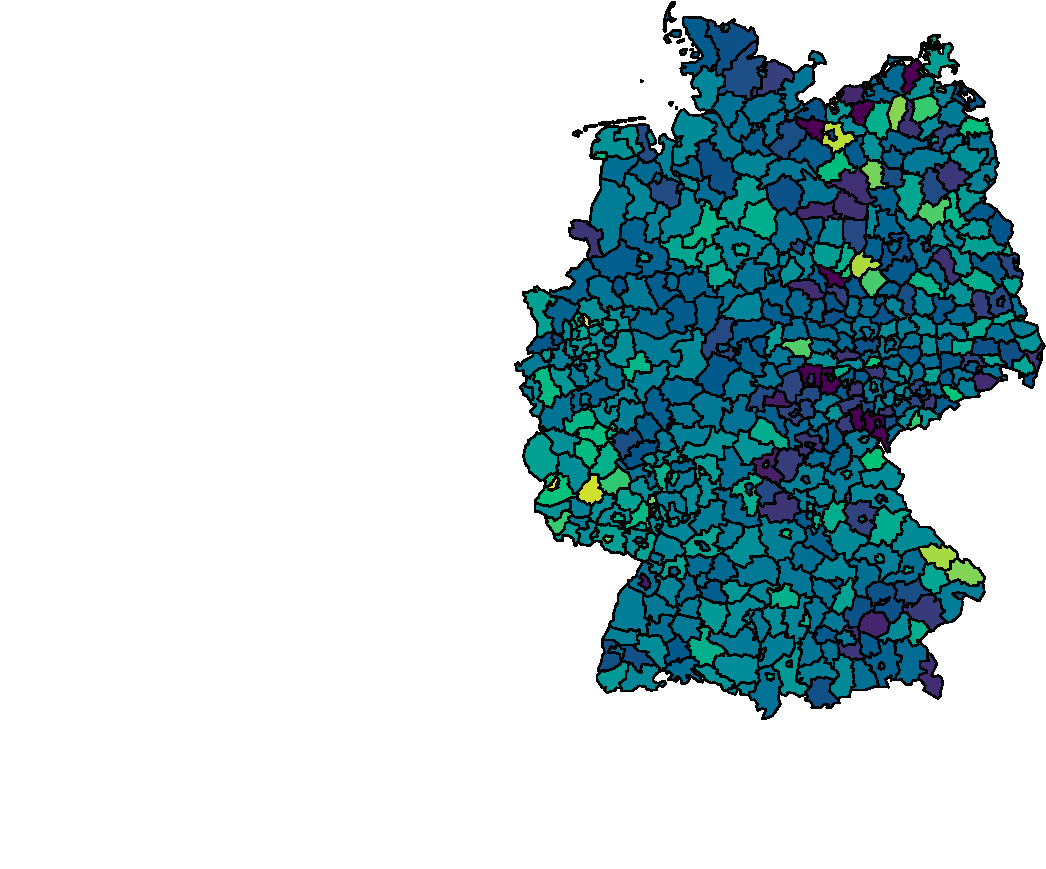
\includegraphics[width=1.1\linewidth]{Part2_RINLA_files/figure-beamer/unnamed-chunk-44-1} \end{center}

\end{col}

\end{cols}
\end{frame}

\begin{frame}{Disease mapping}
\protect\hypertarget{disease-mapping-1}{}
Assume \[
Y_i \mid \eta_i \sim \text{Poisson}(E_i \exp(\eta_i))
\] where the log relative risk is decomposed into \[
\eta_i = \mu + u_i + v_i
\]\\
\strut \\

\begin{itemize}
\item
  \(\mu\) is the overall level (intercept).
\item
  \(v_i \sim \mathcal{N}(0, \tau_v^{-1})\) represents non-spatial
  overdispersion.
\item
  \(u_i\) are random effects with spatial structure.
\end{itemize}
\end{frame}

\begin{frame}{A spatially structured effect}
\protect\hypertarget{a-spatially-structured-effect}{}
To incorporate a spatial structure into a model, the so called
\textcolor{red}{Besag
model} is often used. \[
\begin{aligned}
  p( \bf{u} \mid \kappa_u)& \propto \kappa_u^{(n-1)/2} \exp\left( -
  \frac{\kappa_u}{2} \sum_{i\sim j} (u_i -u_j)^2\right)\\
  & = \kappa_u^{(n-1)/2} \exp\left( -
  \frac{\kappa_u}{2} \bf{u}^T \mathbf{R} \bf{u} \right).
\end{aligned}
\]

where \(R\) is called structure matrix and defined as \[
R_{ij} =  \begin{cases}
            n_i & i=j\\
            -1 & i \sim j\\
            0 & \text{otherwise}.
        \end{cases}
\] Here, \(i \sim j\) denotes that \(i\) and \(j\) are neighbouring
regions.
\end{frame}

\begin{frame}{What does this mean?}
\protect\hypertarget{what-does-this-mean}{}
Example: Five counties of the US state Rhode Island

The structure matrix \(\mathbf{R}\) defines the neighborhood structure.

\begin{cols}

\begin{col}{0.55\textwidth}

\begin{figure}

{\centering 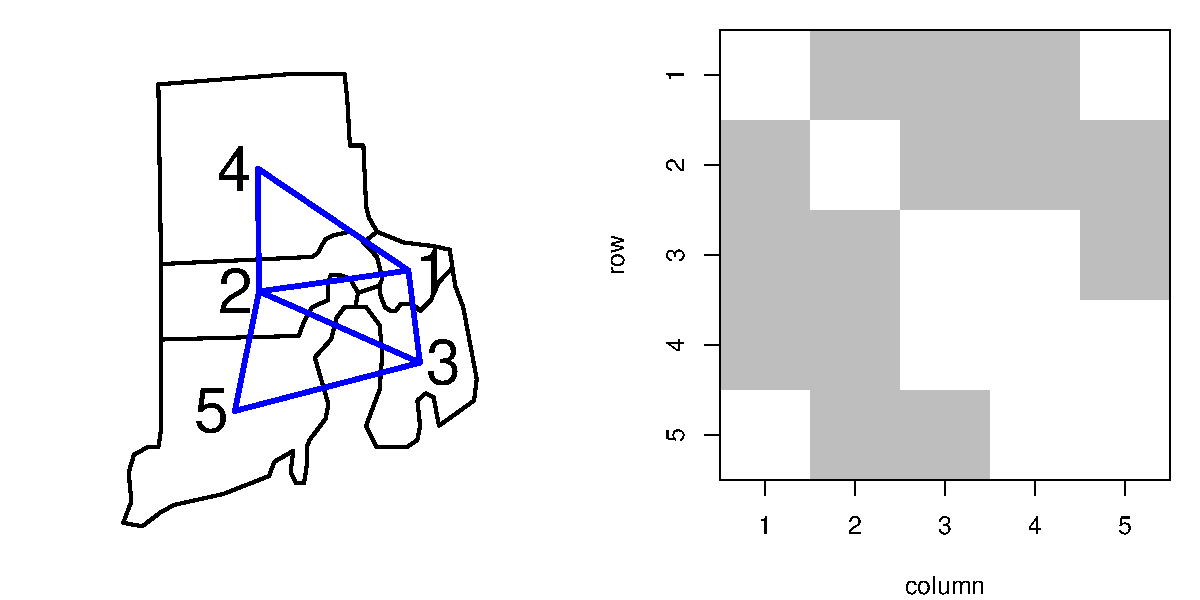
\includegraphics[width=1\linewidth]{graphics/01fig-009} 

}

\caption{Adjacency matrix}\label{fig:unnamed-chunk-45}
\end{figure}

\end{col}

\begin{col}{0.05\textwidth}
~

\end{col}

\begin{col}{0.4\textwidth}

\begin{table}
\begin{tabular}{ccccc}
 \textcolor{red}{3} & -1 & -1 & - 1 & 0 \\
 -1 & \textcolor{red}{4} & -1 & -1 & -1 \\
 -1 & -1 &  \textcolor{red}{3}  & 0 &-1\\
  -1 & -1 & 0 & \textcolor{red}{2} & 0 \\
  0 & -1 & -1 & 0 & \textcolor{red}{2} \\
\end{tabular}
\caption{Structure matrix \textbf{R}}
\end{table}

\end{col}

\end{cols}

With increasing number of regions \(\mathbf{R}\) will be sparse, which
allows to do many computations very efficient.
\end{frame}

\begin{frame}[fragile]{INLA code}
\protect\hypertarget{inla-code}{}
\begin{Shaded}
\begin{Highlighting}[]
\FunctionTok{library}\NormalTok{(spam)}
\CommentTok{\# load the dataset}
\FunctionTok{data}\NormalTok{(Oral)}
\CommentTok{\# load the file including neighbourhood information}
\NormalTok{g }\OtherTok{=} \FunctionTok{system.file}\NormalTok{(}\StringTok{"demodata/germany.graph"}\NormalTok{, }\AttributeTok{package=}\StringTok{"INLA"}\NormalTok{)}
\CommentTok{\# add one column }
\NormalTok{Oral }\OtherTok{=} \FunctionTok{cbind}\NormalTok{(Oral, }\AttributeTok{region =} \DecValTok{1}\SpecialCharTok{:}\DecValTok{544}\NormalTok{, }\AttributeTok{region.unstruc=} \DecValTok{1}\SpecialCharTok{:}\DecValTok{544}\NormalTok{)}
\CommentTok{\# define formula}
\NormalTok{formula }\OtherTok{=}\NormalTok{ Y }\SpecialCharTok{\textasciitilde{}} \FunctionTok{f}\NormalTok{(region, }\AttributeTok{model=}\StringTok{"besag"}\NormalTok{, }\AttributeTok{graph=}\NormalTok{g) }\SpecialCharTok{+}
                           \FunctionTok{f}\NormalTok{(region.unstruc, }\AttributeTok{model=}\StringTok{"iid"}\NormalTok{)}
\CommentTok{\# run the model}
\NormalTok{result }\OtherTok{=} \FunctionTok{inla}\NormalTok{(formula, }\AttributeTok{family=}\StringTok{"poisson"}\NormalTok{, }\AttributeTok{E=}\NormalTok{E, }\AttributeTok{data=}\NormalTok{Oral)}
\end{Highlighting}
\end{Shaded}
\end{frame}

\begin{frame}{Median of \(u\) on exp-scale}
\protect\hypertarget{median-of-u-on-exp-scale}{}
\small

\begin{center}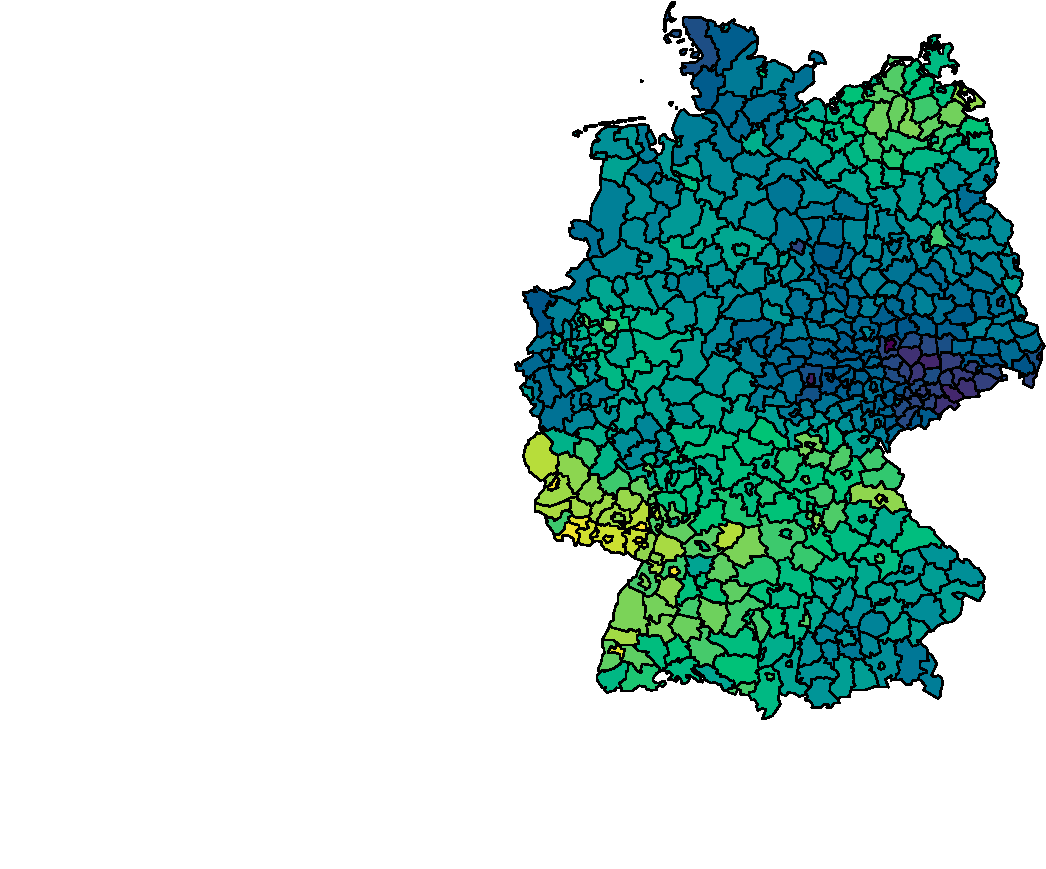
\includegraphics[width=0.6\linewidth]{Part2_RINLA_files/figure-beamer/unnamed-chunk-47-1} \end{center}
\end{frame}

\begin{frame}[fragile]{Other choices for \texttt{f}-terms}
\protect\hypertarget{other-choices-for-f-terms}{}
\small

\begin{verbatim}
##  [1] "linear"       "iid"          "mec"          "meb"          "rgeneric"    
##  [6] "cgeneric"     "rw1"          "rw2"          "crw2"         "seasonal"    
## [11] "besag"        "besag2"       "bym"          "bym2"         "besagproper" 
## [16] "besagproper2" "fgn"          "fgn2"         "ar1"          "ar1c"        
## [21] "ar"           "ou"           "intslope"     "generic"      "generic0"    
## [26] "generic1"     "generic2"     "generic3"     "spde"         "spde2"       
## [31] "spde3"        "iid1d"        "iid2d"        "iid3d"        "iid4d"       
## [36] "iid5d"        "iidkd"        "2diid"        "z"            "rw2d"        
## [41] "rw2diid"      "slm"          "matern2d"     "dmatern"      "copy"        
## [46] "clinear"      "sigm"         "revsigm"      "log1exp"      "logdist"
\end{verbatim}
\end{frame}

\hypertarget{changing-the-prior}{%
\section{Changing the prior}\label{changing-the-prior}}

\begin{frame}[fragile]{Changing the prior: Internal scale}
\protect\hypertarget{changing-the-prior-internal-scale}{}
\begin{itemize}
\tightlist
\item
  Hyperparameters are represented internally with more well-behaved
  transformations, e.g.~correlation \(\rho\) and precision \(\tau\) are
  internally
\end{itemize}

\[
\begin{aligned}
  \theta_1 &= \log(\tau)\\
    \theta_2 &= \log\left(\frac{1+\rho}{1-\rho}\right)
\end{aligned}
\]

\begin{itemize}
\item
  The prior must be set on the parameter in \textbf{internal scale}
\item
  Initial values for the mode-search must be set in \textbf{internal
  scale}
\item
  The functions \texttt{to.theta()} and \texttt{from.theta()} can be
  used to map back and forth.
\end{itemize}
\end{frame}

\begin{frame}[fragile]{Changing the prior: Code}
\protect\hypertarget{changing-the-prior-code}{}
\begin{Shaded}
\begin{Highlighting}[]
\NormalTok{hyper }\OtherTok{=} \FunctionTok{list}\NormalTok{(}\AttributeTok{prec =} \FunctionTok{list}\NormalTok{(}\AttributeTok{prior =} \StringTok{"loggamma"}\NormalTok{,}
                         \AttributeTok{param =} \FunctionTok{c}\NormalTok{(}\DecValTok{1}\NormalTok{, }\FloatTok{0.1}\NormalTok{),}
                         \AttributeTok{initial =} \DecValTok{4}\NormalTok{,}
                         \AttributeTok{fixed =} \ConstantTok{FALSE}\NormalTok{))}

\NormalTok{formula }\OtherTok{=}\NormalTok{ y }\SpecialCharTok{\textasciitilde{}} \FunctionTok{f}\NormalTok{(idx, }\AttributeTok{model =} \StringTok{"iid"}\NormalTok{, }\AttributeTok{hyper =}\NormalTok{ hyper) }\SpecialCharTok{+}\NormalTok{ ...}
\end{Highlighting}
\end{Shaded}

\begin{Shaded}
\begin{Highlighting}[]
\CommentTok{\# For the iid model, default options can be seen with}
\FunctionTok{inla.doc}\NormalTok{(}\StringTok{"iid"}\NormalTok{)}
\end{Highlighting}
\end{Shaded}

\normalsize
\end{frame}

\hypertarget{repeated-poisson-counts}{%
\section{Repeated Poisson counts}\label{repeated-poisson-counts}}

\begin{frame}[fragile]{EPIL example}
\protect\hypertarget{epil-example}{}
Seizure counts in a randomised trial of anti-convulsant therapy in
epilepsy. From \texttt{WinBUGS} manual. \small

\begin{verbatim}
## # A tibble: 6 x 8
##     Ind Repl1 Repl2 Repl3 Repl4   Trt  Base   Age
##   <int> <dbl> <dbl> <dbl> <dbl> <int> <int> <int>
## 1     1     5     3     3     3     0    11    31
## 2     2     3     5     3     3     0    11    30
## 3     3     2     4     0     5     0     6    25
## 4     4     4     4     1     4     0     8    36
## 5     5     7    18     9    21     0    66    22
## 6     6     5     2     8     7     0    27    29
\end{verbatim}

\normalsize

Covariates are treatment (0,1), 8-week baseline seizure counts, and age
in years.
\end{frame}

\begin{frame}[fragile]{Repeated Poisson counts}
\protect\hypertarget{repeated-poisson-counts-1}{}
\[
\begin{aligned}
  y_{jk} & \sim  \text{Poisson}(\mu_{jk});\mbox{  }
        j=1,\dots,59;\; k=1,\dots,4\\
  \log(\mu_{jk})  &= \alpha_0 + \alpha_1
        \log(\text{Base}_j / 4) + \alpha_2\text{Trt}_j\\
    &+ \alpha_3\text{Trt}_j \log(\text{Base}_j / 4) +
        \alpha_4\log(\text{Age}_j) \\
        &+ \alpha_5 V4 + \text{Ind}_j + \beta_{jk}\\
        \alpha_i & \sim  \mathcal{N}(0, \tau_{\alpha})\mbox{   }
        \qquad\tau_{\alpha}\ \  \text{known (0.001)}\\
        \text{Ind}_j & \sim  \mathcal{N}(0, \tau_{\text{Ind}})\quad\tau_{\text{Ind}}\sim\text{Gamma}(1, 0.01)\\
        \beta_{jk} & \sim  \mathcal{N}(0, \tau_{\beta})\mbox{   }
        \qquad\tau_{\beta}\sim\text{Gamma}(1, 0.01)
\end{aligned}
\]

Here, \texttt{V4} is an indicator variable for the 4th visit.
\end{frame}

\begin{frame}[fragile]{Model specification in INLA}
\protect\hypertarget{model-specification-in-inla}{}
The data: \tiny

\begin{verbatim}
##   y Trt Base Age V4 rand Ind
## 1 5   0   11  31  0    1   1
## 2 3   0   11  31  0    2   1
## 3 3   0   11  31  0    3   1
## 4 3   0   11  31  1    4   1
## 5 3   0   11  30  0    5   2
## 6 5   0   11  30  0    6   2
\end{verbatim}

\normalsize

The formula: \footnotesize

\begin{Shaded}
\begin{Highlighting}[]
\NormalTok{formula }\OtherTok{=}\NormalTok{ y }\SpecialCharTok{\textasciitilde{}}\NormalTok{ ClBase4}\SpecialCharTok{*}\NormalTok{CTrt }\SpecialCharTok{+}\NormalTok{ ClAge }\SpecialCharTok{+}\NormalTok{ CV4 }\SpecialCharTok{+}
              \FunctionTok{f}\NormalTok{(Ind, }\AttributeTok{model=}\StringTok{"iid"}\NormalTok{,}
                 \AttributeTok{hyper =} \FunctionTok{list}\NormalTok{(}\AttributeTok{prec =} \FunctionTok{list}\NormalTok{(}\AttributeTok{prior =} \StringTok{"loggamma"}\NormalTok{,}
                 \AttributeTok{param =} \FunctionTok{c}\NormalTok{(}\DecValTok{1}\NormalTok{,}\FloatTok{0.01}\NormalTok{)))) }\SpecialCharTok{+}
              \FunctionTok{f}\NormalTok{(rand, }\AttributeTok{model=}\StringTok{"iid"}\NormalTok{,}
                \AttributeTok{hyper =} \FunctionTok{list}\NormalTok{(}\AttributeTok{prec =} \FunctionTok{list}\NormalTok{(}\AttributeTok{prior =} \StringTok{"loggamma"}\NormalTok{, }
                                         \AttributeTok{param =} \FunctionTok{c}\NormalTok{(}\DecValTok{1}\NormalTok{,}\FloatTok{0.01}\NormalTok{))))}
\end{Highlighting}
\end{Shaded}

\normalsize

Run the model: \footnotesize

\begin{Shaded}
\begin{Highlighting}[]
\NormalTok{result }\OtherTok{=} \FunctionTok{inla}\NormalTok{(formula, }\AttributeTok{family=}\StringTok{"poisson"}\NormalTok{, }\AttributeTok{data =}\NormalTok{ Epil,}
              \AttributeTok{control.fixed =} \FunctionTok{list}\NormalTok{(}\AttributeTok{prec.intercept =} \FloatTok{0.001}\NormalTok{,}
                                   \AttributeTok{prec =} \FloatTok{0.001}\NormalTok{))}
\end{Highlighting}
\end{Shaded}

\normalsize
\end{frame}

\begin{frame}[fragile]{Comparing results with MCMC}
\protect\hypertarget{comparing-results-with-mcmc}{}
\begin{itemize}[<+->]
\tightlist
\item
  When comparing the results of \texttt{R-INLA} with MCMC, it is
  important to use the \textcolor{red}{same model}.
\end{itemize}

That means, same data, same priors, same constraints on parameters,
intercept included or not, \ldots.

\begin{itemize}[<+->]
\tightlist
\item
  Here we have compared the results with those obtained using
  `\texttt{JAGS} via the \texttt{rjags} package
\end{itemize}
\end{frame}

\begin{frame}{}
\protect\hypertarget{section}{}
\begin{center}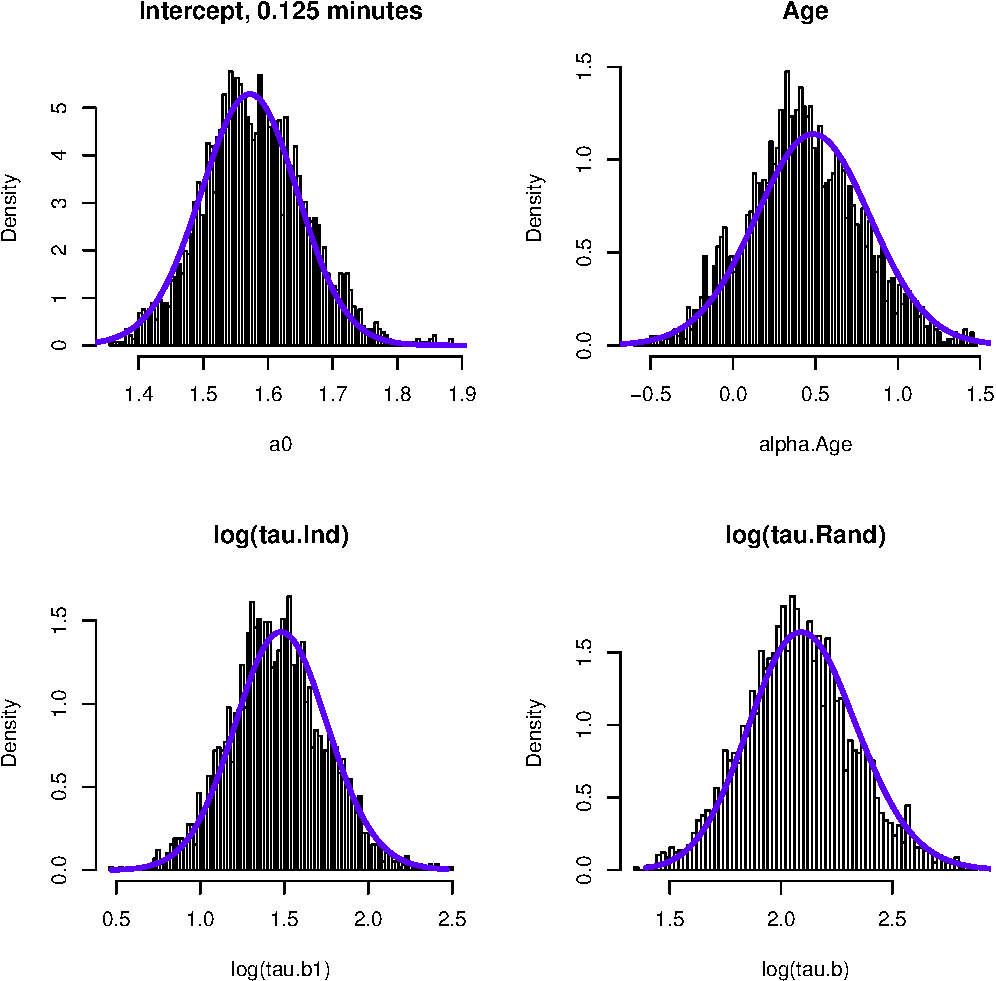
\includegraphics[width=0.7\linewidth]{graphics/results-0125} \end{center}
\scriptsize

Running time of INLA \(<0.5\) seconds \normalsize 
\end{frame}

\begin{frame}{}
\protect\hypertarget{section-1}{}
\begin{center}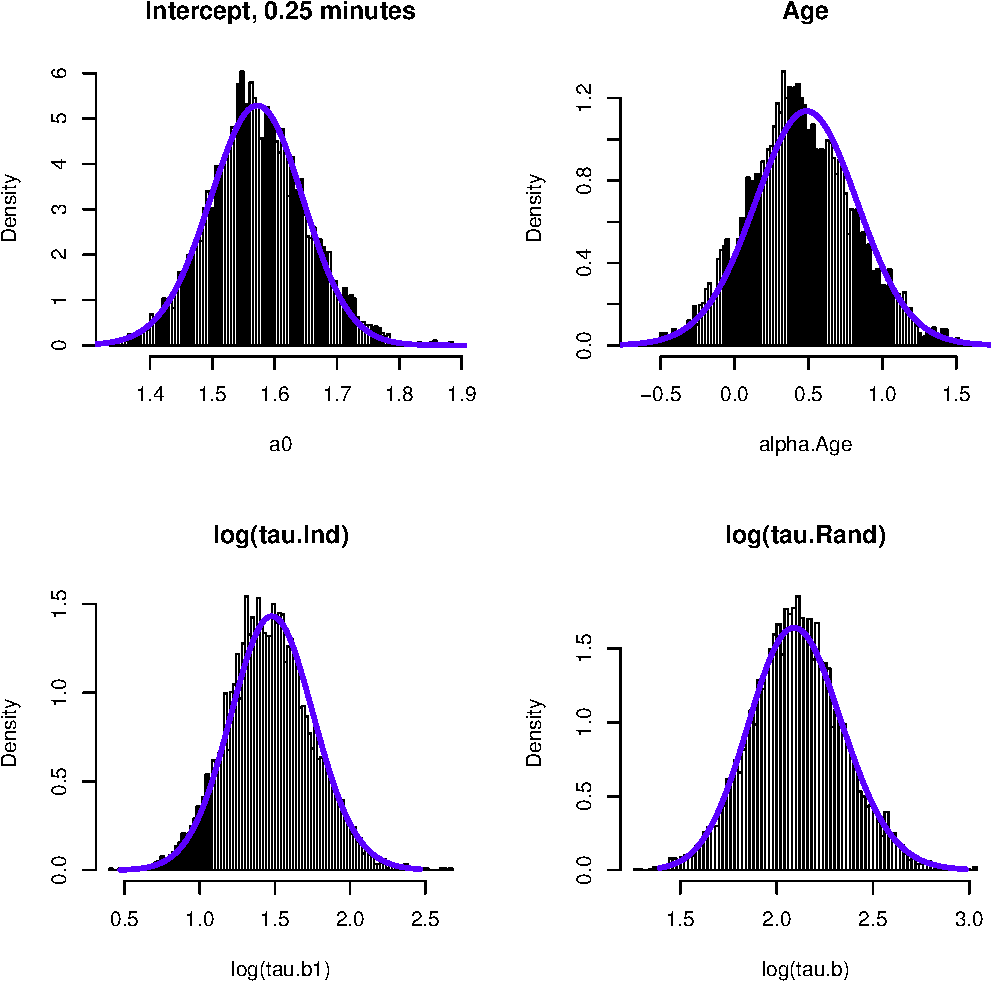
\includegraphics[width=0.7\linewidth]{graphics/results-025} \end{center}
\scriptsize

Running time of INLA \(<0.5\) seconds \normalsize 
\end{frame}

\begin{frame}{}
\protect\hypertarget{section-2}{}
\begin{center}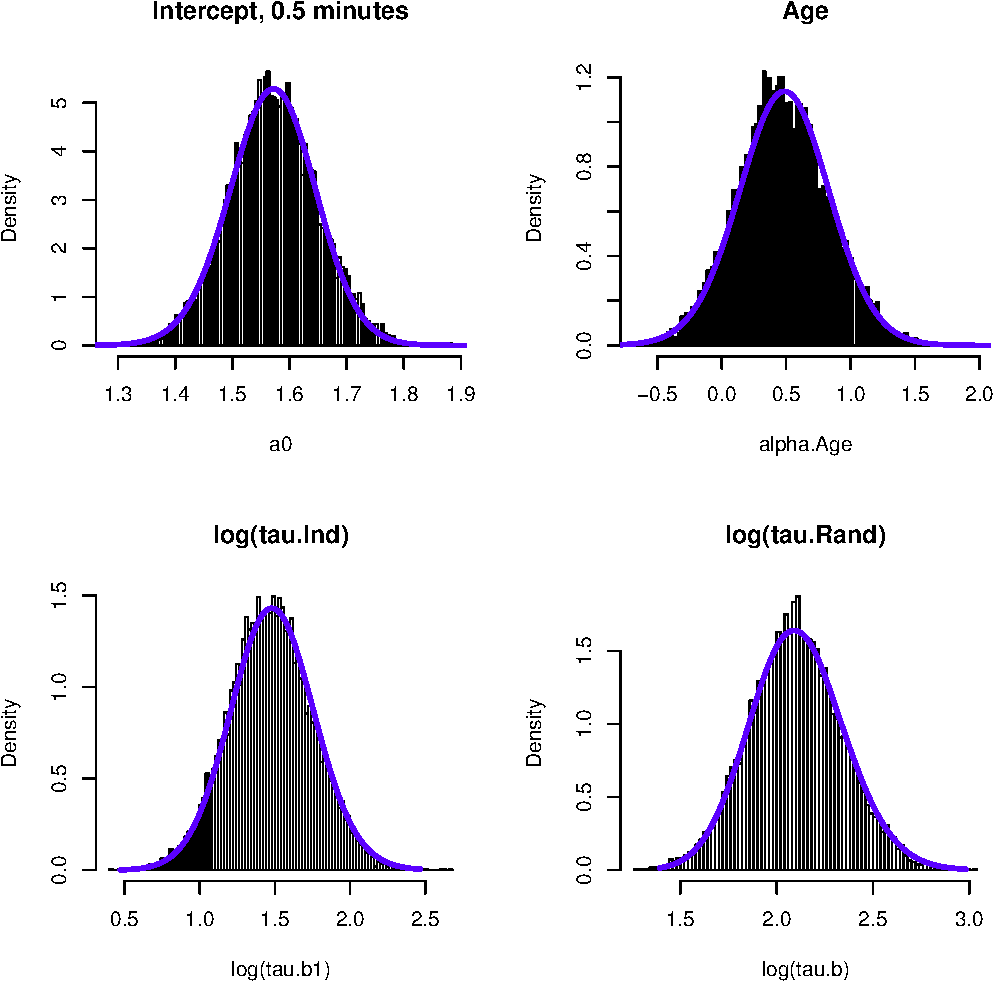
\includegraphics[width=0.7\linewidth]{graphics/results-05} \end{center}
\scriptsize

Running time of INLA \(<0.5\) seconds \normalsize 
\end{frame}

\begin{frame}{}
\protect\hypertarget{section-3}{}
\begin{center}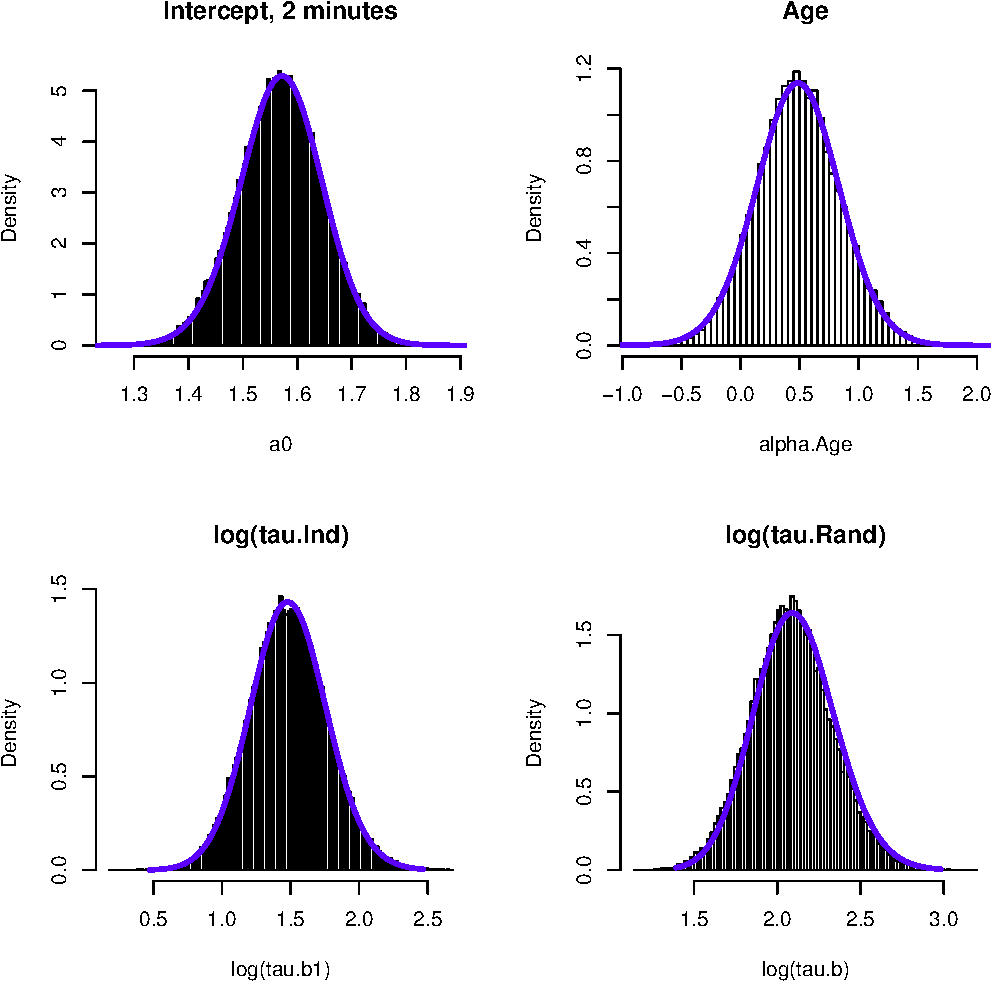
\includegraphics[width=0.7\linewidth]{graphics/results-2} \end{center}
\scriptsize

Running time of INLA \(<0.5\) seconds \normalsize 
\end{frame}

\begin{frame}{}
\protect\hypertarget{section-4}{}
\begin{center}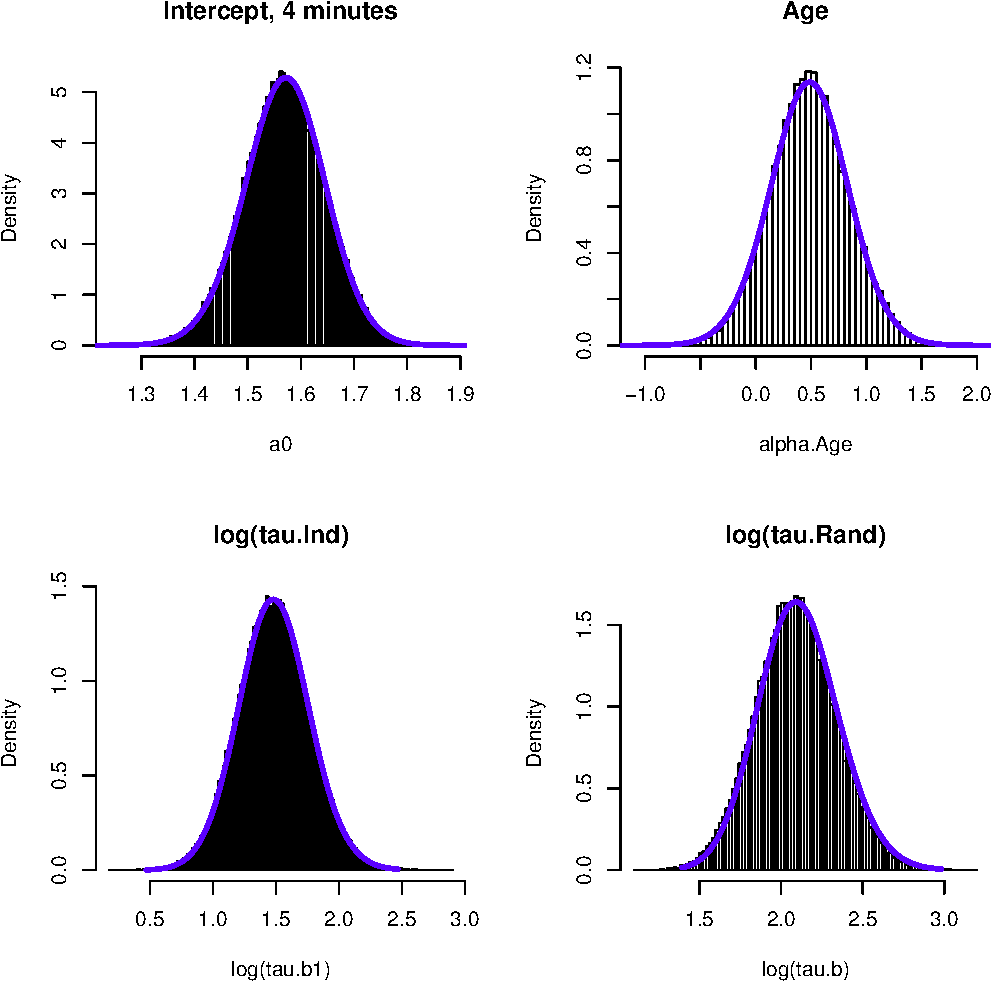
\includegraphics[width=0.7\linewidth]{graphics/results-4} \end{center}
\scriptsize

Running time of INLA \(<0.5\) seconds \normalsize 
\end{frame}

\begin{frame}{}
\protect\hypertarget{section-5}{}
\begin{center}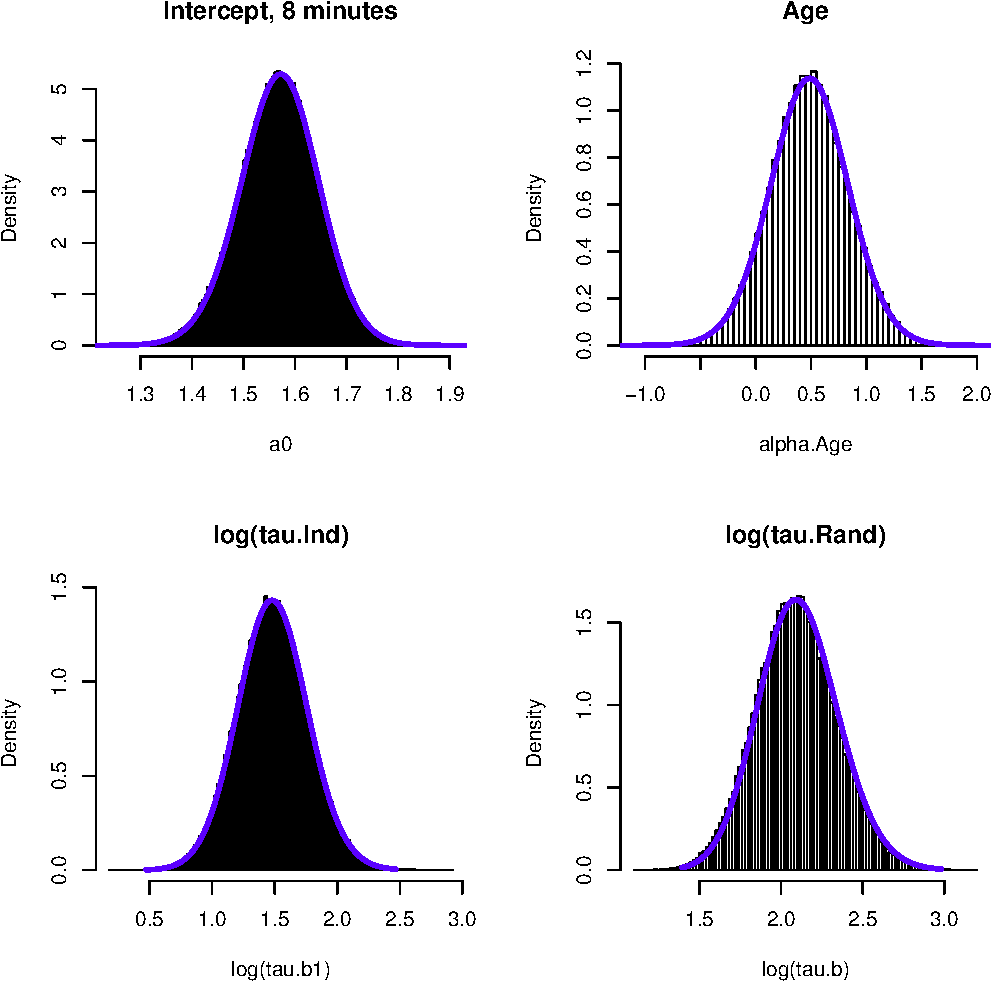
\includegraphics[width=0.7\linewidth]{graphics/results-8} \end{center}
\scriptsize

Running time of INLA \(<0.5\) seconds \normalsize 
\end{frame}

\begin{frame}{}
\protect\hypertarget{section-6}{}
\begin{center}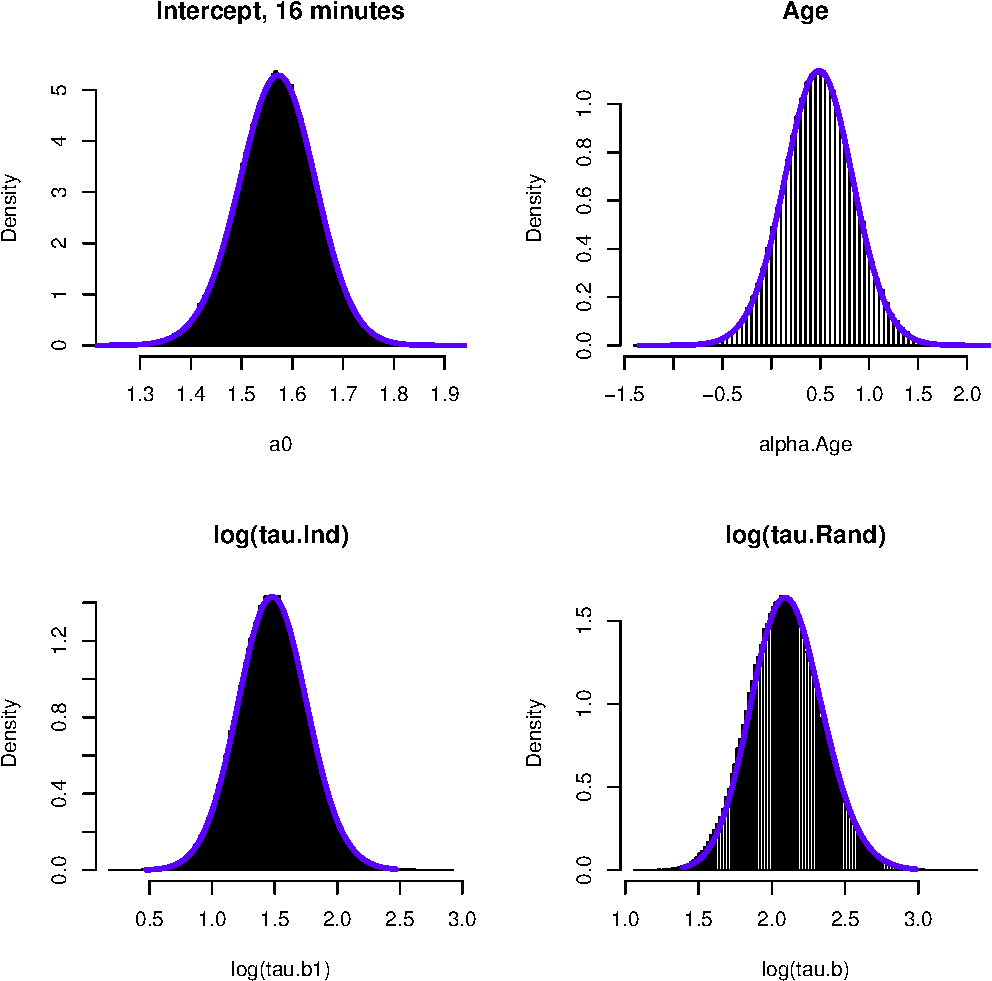
\includegraphics[width=0.7\linewidth]{graphics/results-16} \end{center}
\scriptsize

Running time of INLA \(<0.5\) seconds \normalsize 
\end{frame}

\begin{frame}{}
\protect\hypertarget{section-7}{}
\begin{center}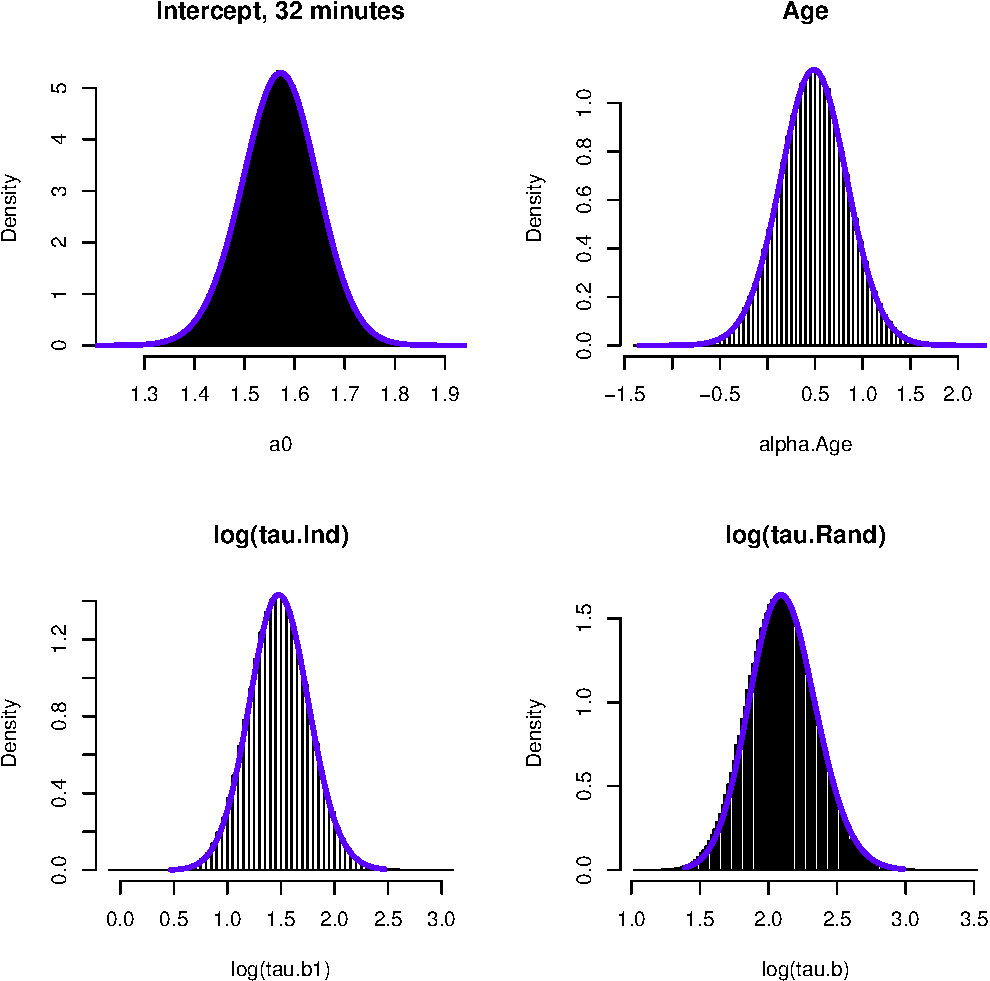
\includegraphics[width=0.7\linewidth]{graphics/results-32} \end{center}
\scriptsize

Running time of INLA \(<0.5\) seconds \normalsize 
\end{frame}

\begin{frame}{}
\protect\hypertarget{section-8}{}
\begin{center}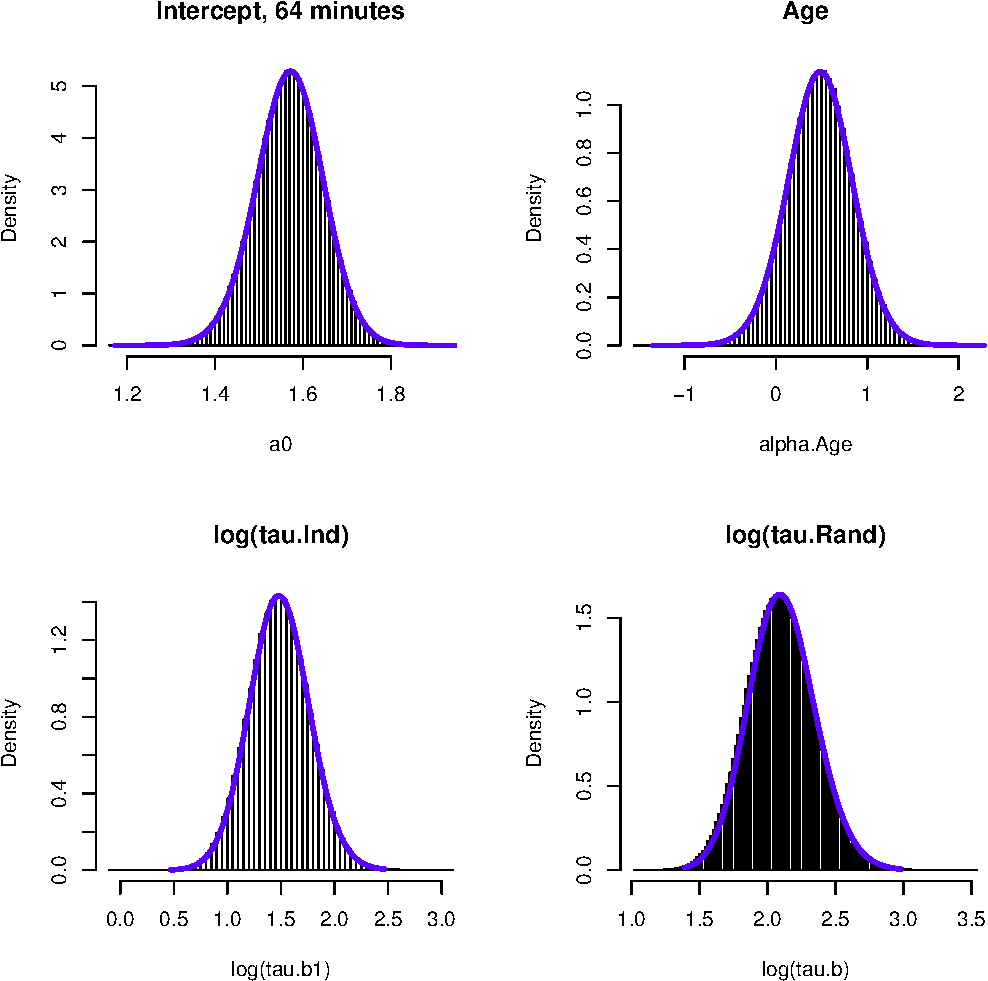
\includegraphics[width=0.7\linewidth]{graphics/results-64} \end{center}
\scriptsize

Running time of INLA \(<0.5\) seconds \normalsize 
\end{frame}

\begin{frame}{}
\protect\hypertarget{section-9}{}
\begin{center}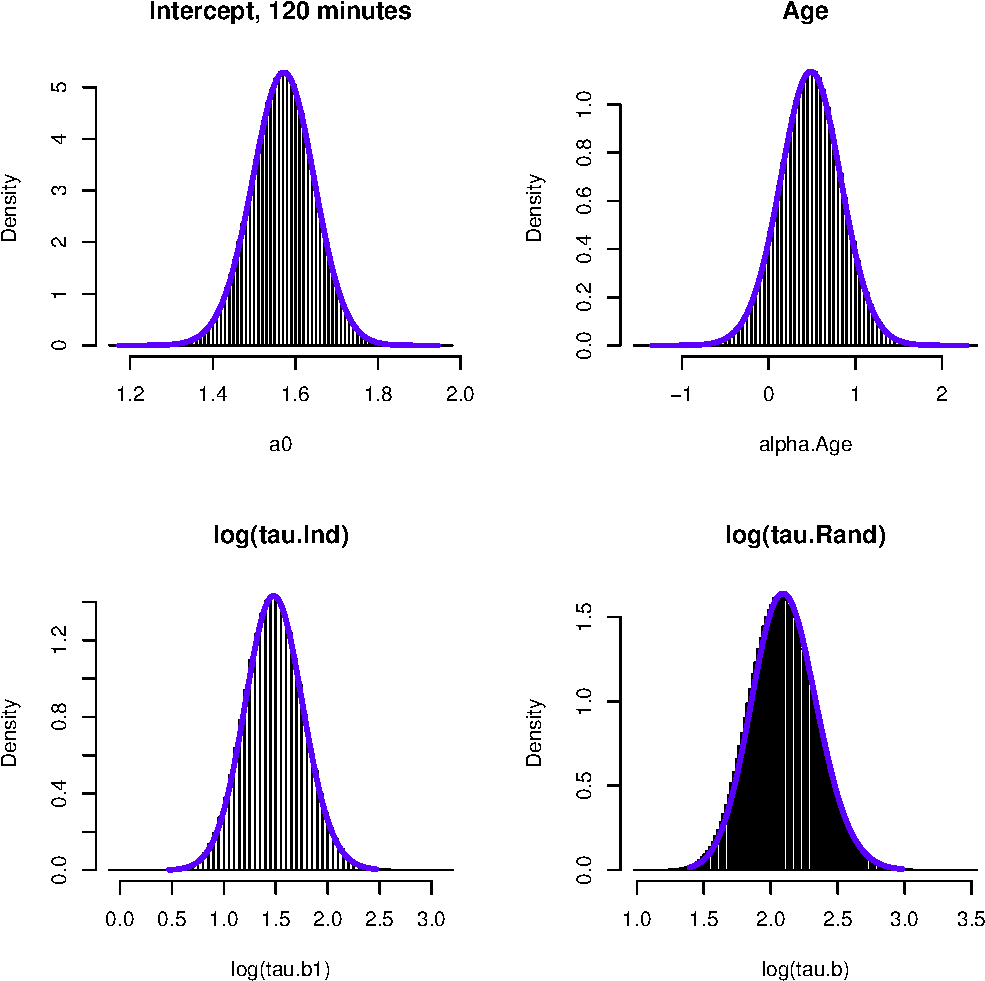
\includegraphics[width=0.7\linewidth]{graphics/results-120} \end{center}
\scriptsize

Running time of INLA \(<0.5\) seconds \normalsize 
\end{frame}

\hypertarget{control-statements}{%
\section{Control statements}\label{control-statements}}

\begin{frame}[fragile]{Control statements}
\protect\hypertarget{control-statements-1}{}
\small

\texttt{control.xxx} statements control computations

\begin{itemize}
\item
  \texttt{control.fixed}

  \begin{itemize}
  \tightlist
  \item
    \texttt{prec}: Default precision for all fixed effects except the
    intercept.
  \item
    \texttt{prec.intercept}: Precision for intercept (Default: 0.0)
  \end{itemize}
\item
  `control.predictor

  \begin{itemize}
  \tightlist
  \item
    \texttt{compute}: Compute posterior marginals of linear predictors
  \end{itemize}
\item
  \texttt{control.compute}

  \begin{itemize}
  \item
    \texttt{dic}, \texttt{mlik}, \texttt{cpo}: Compute measures of fit?

    \begin{itemize}
    \tightlist
    \item
      \texttt{config}: Save internal GMRF approximations? (needed to use
      \texttt{inla.posterior.sample()})
    \end{itemize}
  \end{itemize}
\item
  \texttt{control.inla}

  \texttt{strategy} and \texttt{int.strategy} contain useful advanced
  features
\item
  There are various others as well; see help.
\end{itemize}

\normalsize
\end{frame}

\hypertarget{model-comparison}{%
\section{Model Comparison}\label{model-comparison}}

\begin{frame}[fragile]{Model choice/checking}
\protect\hypertarget{model-choicechecking}{}
There is a need to compare and choose between various models. This is a
difficult problem, but \texttt{R-INLA} has some options available:

\begin{itemize}
\item
  Marginal likelihood \(\Rightarrow\) Bayes factors
\item
  Deviance information criterion (DIC)
\item
  Widely applicable information criterion (WAIC)\\
  \strut \\
  There are also some predictive checks for the model:
\item
  Conditional predictive ordinate (CPO)
\item
  Probability integral transform (PIT)
\end{itemize}
\end{frame}

\begin{frame}[fragile]{Marginal likelihood}
\protect\hypertarget{marginal-likelihood}{}
\small

\begin{Shaded}
\begin{Highlighting}[]
\NormalTok{result }\OtherTok{=} \FunctionTok{inla}\NormalTok{(formula,}
              \AttributeTok{data =}\NormalTok{ data,}
              \AttributeTok{control.compute=}\FunctionTok{list}\NormalTok{(}\AttributeTok{mlik=}\ConstantTok{TRUE}\NormalTok{))}
\CommentTok{\# See result}
\NormalTok{result}\SpecialCharTok{$}\NormalTok{mlik}
\end{Highlighting}
\end{Shaded}

\normalsize

\begin{itemize}
\item
  Calculates \(\log(\pi(\boldsymbol{y}))\)
\item
  Can calculate Bayes factors through differences in value
\item
  \textbf{NB:} Problematic for intrinsic models
\end{itemize}
\end{frame}

\begin{frame}[fragile]{Deviance information criterion}
\protect\hypertarget{deviance-information-criterion}{}
\small

\begin{Shaded}
\begin{Highlighting}[]
\NormalTok{result }\OtherTok{=} \FunctionTok{inla}\NormalTok{(formula,}
              \AttributeTok{data =}\NormalTok{ data,}
              \AttributeTok{control.compute=}\FunctionTok{list}\NormalTok{(}\AttributeTok{dic=}\ConstantTok{TRUE}\NormalTok{))}

\CommentTok{\# See result}
\NormalTok{result}\SpecialCharTok{$}\NormalTok{dic}\SpecialCharTok{$}\NormalTok{dic}
\end{Highlighting}
\end{Shaded}

\normalsize

\hfill\break
\hfill\break
DIC is a measure of complexity and fit. It is used to compare complex
hierarchical models and is defined as:

\[
\text{DIC} = \overline{D} + p_D
\]

where \(\overline{D}\) is the posterior mean of the deviance and \(p_D\)
is the effective number of parameters. Smaller values of the DIC
indicate a better trade-off between complexity and fit of the model.
\end{frame}

\begin{frame}[fragile]{Widely applicable information criterion (WAIC)}
\protect\hypertarget{widely-applicable-information-criterion-waic}{}
\small

\begin{Shaded}
\begin{Highlighting}[]
\NormalTok{result }\OtherTok{=} \FunctionTok{inla}\NormalTok{(formula,}
              \AttributeTok{data =}\NormalTok{ data,}
              \AttributeTok{control.compute=}\FunctionTok{list}\NormalTok{(}\AttributeTok{waic=}\ConstantTok{TRUE}\NormalTok{))}

\CommentTok{\# See result}
\NormalTok{result}\SpecialCharTok{$}\NormalTok{waic}\SpecialCharTok{$}\NormalTok{waic}
\end{Highlighting}
\end{Shaded}

\normalsize

\begin{itemize}
\item
  WAIC is like DIC just newer, and perhaps better
\item
  See \emph{``Understanding predictive information criteria for Bayesian
  models''} (2013) by Andrew Gelman, Jessica Hwang, and Aki Vehtari
\end{itemize}
\end{frame}

\begin{frame}[fragile]{Conditional predictive ordinate}
\protect\hypertarget{conditional-predictive-ordinate}{}
\small

\begin{Shaded}
\begin{Highlighting}[]
\NormalTok{result }\OtherTok{=} \FunctionTok{inla}\NormalTok{(formula,}
              \AttributeTok{data =}\NormalTok{ data,}
              \AttributeTok{control.compute=}\FunctionTok{list}\NormalTok{(}\AttributeTok{cpo=}\ConstantTok{TRUE}\NormalTok{))}

\CommentTok{\# See result}
\NormalTok{result}\SpecialCharTok{$}\NormalTok{cpo}\SpecialCharTok{$}\NormalTok{cpo}
\end{Highlighting}
\end{Shaded}

\normalsize

\begin{itemize}
\item
  Measures fit through the predictive density
  \(\pi(y_i^{obs}\mid\boldsymbol{y}_{-i})\)
\item
  Basically, Bayesian hold-one out
\item
  Easy to compute in the INLA-approach
\item
  Possible failure (\$cpo\$failure)
\item
  See \emph{Posterior and Cross-validatory Predictive Checks: A
  Comparison of MCMC and INLA} (2009) by Held, Schr\{"o\}dle and Rue
\end{itemize}
\end{frame}

\begin{frame}[fragile]{Probability integral transform}
\protect\hypertarget{probability-integral-transform}{}
\small

\begin{Shaded}
\begin{Highlighting}[]
\NormalTok{result }\OtherTok{=} \FunctionTok{inla}\NormalTok{(formula,}
              \AttributeTok{data =}\NormalTok{ data,}
              \AttributeTok{control.compute=}\FunctionTok{list}\NormalTok{(}\AttributeTok{cpo=}\ConstantTok{TRUE}\NormalTok{))}

\CommentTok{\# See result}
\NormalTok{result}\SpecialCharTok{$}\NormalTok{cpo}\SpecialCharTok{$}\NormalTok{pit}
\end{Highlighting}
\end{Shaded}

\normalsize

\begin{itemize}
\tightlist
\item
  Given by
\end{itemize}

\[
\text{Prob}(Y_i \leq y_i^{obs} \mid \boldsymbol{y}_{-i})
\]

\begin{itemize}
\item
  Detects outliers
\item
  Should look out for unusually small or large values
\item
  PIT histograms should be uniform
\end{itemize}
\end{frame}

\begin{frame}{Model choice: Recap}
\protect\hypertarget{model-choice-recap}{}
\begin{itemize}
\item
  Information Criteria or predictive checks essentially for free
\item
  But they may not be appropriate
\end{itemize}
\end{frame}

\begin{frame}{}
\protect\hypertarget{section-10}{}
\Large

Thank you for your attention!

\normalsize

If you have any doubts or questions, please write :
\url{sara.martino@math.ntnu.no}

\begin{center}
\includegraphics[width=0.3\linewidth]{graphics/smiley_small} \end{center}
\end{frame}

\end{document}
